%%%%%%%%%%%%%%%%%%%%%%%%%%%%%%%%%%%%%%%%%%%%%%%%%%%%%%%%%%%%%%%%%%%%%%%
% Vorlage für Bachelor- und Masterarbeiten mit pdflatex nach dem Layout des ITS
% Fabian Bleier (fabian.bleier@kit.edu), September 2016
%%%%%%%%%%%%%%%%%%%%%%%%%%%%%%%%%%%%%%%%%%%%%%%%%%%%%%%%%%%%%%%%%%%%%%%
% Kurzbeschreibung
% Der Hauptordner enthält in erster Linie das Dokument "gesamt.tex". Dieses enthält wiederum alle notwendigen Nutzereingaben (Autor, Titel etc.). 
% Die einzelnen Kapitel werden in das Gesamtdokument eingeladen und liegen im Ordner "kapitel". 
% Der Ordner "sonstiges" enthält alle Seiten außerhalb des eigentlichen Textkörpers (Formatierung der Kopfzeilen, Deckblätter, die einzubindenden Pakete, Institutslogos, Macros, Verzeichnisse usw.)
% Der Ordner "literatur" enthält alle Dateien, welche zur Gestaltung eines Literaturverzeichnisses notwendig sind (Die bibtex-Datei, die bst-Datei, und das eigentliche Verzeichnis).
% Im Ordner "bilder" können alle Abbildungen abgelegt werden.
 % Der Ordner "dokumentation" enthält verschiedene Dokumentationen zu den verwendeten Paketen, ferner eine ausbaufähige Dokumentation des LaTeX-Dokuments

%%%%%%%%%%%%%%%%%%%%%%%%%%%%%%%%%%%%%%%%%%%%%%%%%%%%%%%%%%%%%%%%%%%%%%%
% Dokumenterstellung
%%%%%%%%%%%%%%%%%%%%%%%%%%%%%%%%%%%%%%%%%%%%%%%%%%%%%%%%%%%%%%%%%%%%%%%
\documentclass[
paper=a4,										% Seitenformat
12pt,											% Schriftgröße
twoside=false,									% zweiseitig true/false
headings=small,									% Formatierung der Überschriften
draft=false,									% Entwurfsmodus true/false
]{scrreprt}										% KOMA-Klasse Report
%\usepackage{showframe}							% Schriftfeld in Dokument anzeigen

%%%%%%%%%%%%%%%%%%%%%%%%%%%%%%%%%%%%%%%%%%%%%%%%%%%%%%%%%%%%%%%%%%%%%%%
% Metadaten und Variablen zur Verwendung im Dokument und zur Erstellung der PDF-Datei
%%%%%%%%%%%%%%%%%%%%%%%%%%%%%%%%%%%%%%%%%%%%%%%%%%%%%%%%%%%%%%%%%%%%%%%
\newcommand{\doctitle}{} 				% Titel der Arbeit
\newcommand{\doctype}{}			% Dokumenttyp
\newcommand{\docauthor}{}	% Autor
\newcommand{\doclocation}{Karlsruhe}			% Erstellungsort
\newcommand{\betreuerI}{}	% Betreuer1
\newcommand{\betreuerII}{}						% Betreuer2 (optional, kann leer gelassen werden)												
\newcommand{\doccreator}{pdflatex}				% Erstellt mit
\newcommand{\docproducer}{LaTeX}				% Software
\newcommand{\docdate}{\today}					% Erstellungsdatum

%%%%%%%%%%%%%%%%%%%%%%%%%%%%%%%%%%%%%%%%%%%%%%%%%%%%%%%%%%%%%%%%%%%%%%%
% Formatierung, Pakete, Makros einbinden
%%%%%%%%%%%%%%%%%%%%%%%%%%%%%%%%%%%%%%%%%%%%%%%%%%%%%%%%%%%%%%%%%%%%%%%
%%%%%%%%%%%%%%%%%%%%%%%%%%%%%%%%%%%%%%%%%%%%%%%%%%%%%%%%%%%%%%%%%%%%%%%%%%%%%%%%%%%%%%%%
% Standardpakete
% Hilfe zu Paketen bieten die Kommandozeilentools texdoc (TeXLive) bzw. mthelp (Miktex)
%%%%%%%%%%%%%%%%%%%%%%%%%%%%%%%%%%%%%%%%%%%%%%%%%%%%%%%%%%%%%%%%%%%%%%%%%%%%%%%%%%%%%%%%
\usepackage[comma,
	sort, square, 	numbers
	]{natbib}									% Formatierung des Literaturverzeichnisses 
\usepackage[ngerman,english]{babel} 			% Sprachpaket: neudeutsch, englisch, französisch
\usepackage[utf8]{inputenc}        				% Standardpackage: unterstützt Zeichentabellen
\usepackage[T1]{fontenc}              			% Standardpackage: unterstützt Schriftauswahl
\usepackage{lmodern}							% Schrift latin modern
\usepackage{amsmath}                  			% Standardpackage: Formelformatierung
\usepackage{amsfonts}                 			% Standardpackage: Formelformatierung
\usepackage{amssymb}                  			% Standardpackage: Formelformatierung
\usepackage{mathptmx}   						% Formeln und Text mit Adobe Times Roman Postscript-Schriften
\usepackage[scaled=.92]{helvet}					% Helvetica ist serifenlose Standardschriftart
\usepackage{courier}							% Courier ist typeset Standardschriftart
\usepackage{fixmath}   							% ISO-Formatierung griechischer Buchstaben
\usepackage[headsepline
	]{scrlayer-scrpage}							% Header-Formatierung
\usepackage{siunitx}                  			% Formatierung der Einheiten
\sisetup{
	per-mode=symbol,							% Form des Bruchstrichs: reciprocal (Exponent), symbol (/) oder fraction
	locale = DE 								% Ländereinstellung (Dezimaltrennzeichen usw.)
}
\usepackage{graphicx}							% Zusätzliche Optionen zur Grafikeinbindung
%\graphicspath{{./bilder/}]}

%%%%%%%%%%%%%%%%%%%%%%%%%%%%%%%%%%%%%%%%%%%%%%%%%%%%%%%%%%%%%%%%%%%%%%%%%%%%%%%%%%
% Zusätzliche Pakete
%%%%%%%%%%%%%%%%%%%%%%%%%%%%%%%%%%%%%%%%%%%%%%%%%%%%%%%%%%%%%%%%%%%%%%%%%%%%%%%%%%
\usepackage[
	margin=10pt,
	labelformat=simple,
	labelsep=colon,
	font=normal,
	labelfont=normal,
	skip=15pt
	]{caption}[2008/08/24]  					% Erlaubt die Formatierung der Bildunter- und Tabellenüberschriften
\usepackage{ifthen}								% Paket für Abfragen
\usepackage{color}								% Farbige Texte
\usepackage{transparent}						% Transparenz
\usepackage{booktabs}							% Nützliche Tabellentools (\topline, \midline, \bottomline, ...)
\usepackage{longtable}							% Tabellen über mehrere Seiten

%%%%%%%%%%%%%%%%%%%%%%%%%%%%%%%%%%%%%%%%%%%%%%%%%%%%%%%%%%%%%%%%%%%%%%%%%%%%%%%%%%
% Optionale (aber evtl. nützliche) Pakete
%%%%%%%%%%%%%%%%%%%%%%%%%%%%%%%%%%%%%%%%%%%%%%%%%%%%%%%%%%%%%%%%%%%%%%%%%%%%%%%%%%
\usepackage{lipsum}								% Einbindung von Lorem Ipsum als Platzhalter
\usepackage{multirow}                 			% Befehle analog \multicolumn in vertikaler Richtung
\usepackage{subcaption}							% Ermöglicht die Verwendung von subfigure
\PreventPackageFromLoading{subfig} 				% Verhindert das Laden des veralteten Packages subfig
\usepackage[hyphens]{url}
\usepackage[svgpath=bilder/]{svg}	  			% Automatisches Einbinden von svg-Dateien
\usepackage{textcomp}							% Ermöglicht die Einbindung von Symbolen
\usepackage[
	colorlinks=true, 
	linkcolor=black, 
	citecolor=black, 
	urlcolor=black
	]{hyperref}									% Verlinkte Referenzen
%\hypersetup{
%	pdftitle={\doctitle},
	%pdfsubject={\docsubject},
	%pdfauthor={\docauthor},
	%pdfkeywords={\dockeywords},
  %pdfcreator={\doccreator},
  %pdfproducer={\docproducer}
%}
\usepackage{nameref}							% Definition der Metadaten, die dem PDF-Dokument hinterlegt werden
\usepackage[nonumberlist,
	nomain=true,
	acronym,
	toc,
	numberedsection=false,
	]{glossaries}								% Glossaries-Paket zur Erstellung eines Glossars
\newcounter{dummy} 								% korrekte Verlinkung der Literatur und anderer Verzeichnisse

%comments and notes https://tex.stackexchange.com/questions/9796/how-to-add-todo-notes
\usepackage[colorinlistoftodos,prependcaption,textsize=tiny]{todonotes}
\newcommand{\unsure}[2][1=]{\todo[linecolor=red,backgroundcolor=red!25,bordercolor=red,#1]{#2}}
\newcommand{\change}[2][1=]{\todo[linecolor=blue,backgroundcolor=blue!25,bordercolor=blue,#1]{#2}}
\newcommand{\info}[2][1=]{\todo[linecolor=OliveGreen,backgroundcolor=OliveGreen!25,bordercolor=OliveGreen,#1]{#2}}
\newcommand{\improvement}[2][1=]{\todo[linecolor=Plum,backgroundcolor=Plum!25,bordercolor=Plum,#1]{#2}}
\newcommand{\thiswillnotshow}[2][1=]{\todo[disable,#1]{#2}}
\usepackage{listings}
\usepackage{color}

\definecolor{dkgreen}{rgb}{0,0.6,0}
\definecolor{gray}{rgb}{0.5,0.5,0.5}
\definecolor{mauve}{rgb}{0.58,0,0.82}

\lstset{frame=none,
  language=[Sharp]C,
  aboveskip=3mm,
  belowskip=3mm,
  showstringspaces=false,
  columns=flexible,
  basicstyle={\small\ttfamily},
  numbers=left,
  stepnumber=1,
  keywordstyle=\color{blue},
  commentstyle=\color{dkgreen},
  stringstyle=\color{mauve},
  breaklines=false,
  breakatwhitespace=true,
  tabsize=3
}					% Pakete
%%%%%%%%%%%%%%%%%%%%%%%%%%%%%%%%%%%%%%%%%%%%%%%%%%%%%%%%%%%%%%%%%%%%%%%
% Zuweisen von Zahlenwerten zu Monatsnamen 
%%%%%%%%%%%%%%%%%%%%%%%%%%%%%%%%%%%%%%%%%%%%%%%%%%%%%%%%%%%%%%%%%%%%%%%
\newcommand{\monthword}[1]{\ifcase#1\or Januar\or Februar\or M\"arz\or April\or
                                        Mai\or Juni\or Juli\or August\or
                                        September\or Oktober\or November\or Dezember\fi}
																				
%%%%%%%%%%%%%%%%%%%%%%%%%%%%%%%%%%%%%%%%%%%%%%%%%%%%%%%%%%%%%%%%%%%%%%%%%%%%%%%%%%%%%%%%%
% Benutzerdefinierte Übersetzungen (Fixed names und Variablen)
%%%%%%%%%%%%%%%%%%%%%%%%%%%%%%%%%%%%%%%%%%%%%%%%%%%%%%%%%%%%%%%%%%%%%%%%%%%%%%%%%%%%%%%%%
% Definieren von neuen Namen für die einzelnen Tabellen
\newcommand{\latinsymbolsname}{}
\newcommand{\greeksymbolsname}{}
\newcommand{\indicesname}{}
\newcommand{\simparsname}{}
\newcommand{\abbrevsname}{}
\newcommand{\unitname}{}
\newcommand{\descname}{}
% ngerman
\addto\captionsngerman{
  \renewcommand{\indexname}{Symbolverzeichnis}
  \renewcommand{\refname}{Literaturverzeichnis}
	\renewcommand{\latinsymbolsname}{Lateinische~Symbole}
	\renewcommand{\greeksymbolsname}{Griechische~Symbole}
	\renewcommand{\indicesname}{Indizes}
	\renewcommand{\simparsname}{Ähnlichkeitskennzahlen}
	\renewcommand{\abbrevsname}{Abkürzungen}
	\renewcommand{\symbolname}{Formelzeichen}
	\renewcommand{\unitname}{Einheit}
	\renewcommand{\descname}{Beschreibung}
}
% german (Verwendung wird nicht empfohlen)
\addto\captionsgerman{
  \renewcommand{\indexname}{Symbolverzeichnis}
  \renewcommand{\refname}{Literaturverzeichnis}
	\renewcommand{\latinsymbolsname}{Lateinische~Symbole}
	\renewcommand{\greeksymbolsname}{Griechische~Symbole}
	\renewcommand{\indicesname}{Indizes}
	\renewcommand{\simparsname}{Ähnlichkeitskennzahlen}
	\renewcommand{\abbrevsname}{Abkürzungen}
	\renewcommand{\symbolname}{Formelzeichen}
	\renewcommand{\unitname}{Einheit}
	\renewcommand{\descname}{Beschreibung}
}
% english (Verwendung wird nicht empfohlen)
\addto\captionsenglish{
  \renewcommand{\indexname}{List of Symbols}
  \renewcommand{\latinsymbolsname}{Latin~symbols}
	\renewcommand{\greeksymbolsname}{Greek~symbols}
	\renewcommand{\indicesname}{Indices}
	\renewcommand{\simparsname}{Similarity parameters}
	\renewcommand{\abbrevsname}{Abbreviations}
	\renewcommand{\symbolname}{Symbol}
	\renewcommand{\unitname}{Unit}
	\renewcommand{\descname}{Description}
}
% french (Verwendung wird nicht empfohlen)
\addto\captionsfrench{
  \renewcommand{\indexname}{Table de Symboles}
  \renewcommand{\latinsymbolsname}{Lettres~latines}
	\renewcommand{\greeksymbolsname}{Lettres~grecques}
	\renewcommand{\indicesname}{Indices}
	\renewcommand{\simparsname}{Nombres sans dimension}
	\renewcommand{\abbrevsname}{Abréviations}
	\renewcommand{\symbolname}{Symbol}
	\renewcommand{\unitname}{Unité}
	\renewcommand{\descname}{Description}
}

%%%%%%%%%%%%%%%%%%%%%%%%%%%%%%%%%%%%%%%%%%%%%%%%%%%%%%%%%%%%%%%%%%%%%%%%%%%%%%%%%%%%%%%%%%
%% Glossardateien erstellen
%%%%%%%%%%%%%%%%%%%%%%%%%%%%%%%%%%%%%%%%%%%%%%%%%%%%%%%%%%%%%%%%%%%%%%%%%%%%%%%%%%%%%%%%%%
%% Indexdateien für Symbolverzeichnis erstellen
%% \newglossary[Dateiendung Protokolldatei]{Typ des Glossars}{Dateiendung für Eingabedatei VOR Verarbeitung}{Dateiendung für Eingabedatei NACH Verarbeitung}{Titel}
%\newglossary[slg1]{latinSymb}{syi1_temp}{syg1}{\latinsymbolsname}
%\newglossary[slg2]{greekSymb}{syi2_temp}{syg2}{\greeksymbolsname}
%\newglossary[slg3]{simPar}{syi3_temp}{syg3}{\simparsname}
%\newglossary[slg4]{indices}{syi4_temp}{syg4}{\indicesname}
%\newglossary[slg5]{abbrevs}{syi5_temp}{syg5}{\abbrevsname}
%% Hinzufügen des Eintrags unit{}, damit eine Einheit angegeben werden kann.
%\glsaddkey{unit}{\glsentrytext{\glslabel}}{\glsentryunit}{\GLsentryunit}{\glsunit}{\Glsunit}{\GLSunit}
%\makeglossaries					% Selbstgeschriebene Macros
%%%%%%%%%%%%%%%%%%%%%%%%%%%%%%%%%%%%%%%%%%%%%%%%%%%%%%%%%%%%%%%%%%%%%%%%%%%%%%%%%%%%%%%%%
% Allgemein
%%%%%%%%%%%%%%%%%%%%%%%%%%%%%%%%%%%%%%%%%%%%%%%%%%%%%%%%%%%%%%%%%%%%%%%%%%%%%%%%%%%%%%%%%
\setlength{\unitlength}{1truecm}					% Maßeinheit fuer Bildgroessen etc. 1cm
\hyphenation{} 	% Trennhilfen einfügen

%%%%%%%%%%%%%%%%%%%%%%%%%%%%%%%%%%%%%%%%%%%%%%%%%%%%%%%%%%%%%%%%%%%%%%%%%%%%%%%%%%%%%%%%%
% Unterdrückung von Warnmeldungen (insbesondere 'overfull boxes')
%%%%%%%%%%%%%%%%%%%%%%%%%%%%%%%%%%%%%%%%%%%%%%%%%%%%%%%%%%%%%%%%%%%%%%%%%%%%%%%%%%%%%%%%%
\hfuzz2pt
\vfuzz6pt
\hbadness=10000
\vbadness=10000
%\pdfsuppresswarningpagegroup=1

%%%%%%%%%%%%%%%%%%%%%%%%%%%%%%%%%%%%%%%%%%%%%%%%%%%%%%%%%%%%%%%%%%%%%%%%%%%%%%%%%%%%%%%%%
% Textspiegel
%%%%%%%%%%%%%%%%%%%%%%%%%%%%%%%%%%%%%%%%%%%%%%%%%%%%%%%%%%%%%%%%%%%%%%%%%%%%%%%%%%%%%%%%%
\setlength{\headheight}{18pt}     					% Höhe der Kopfzeile
\setlength{\textheight}{24.0cm}              		% Texthöhe
\setlength{\textwidth}{16.0cm}               		% Textbreite
\setlength{\topmargin}{-1.0cm}               		% oberen Seitenrand festlegen, bzw. verschieben
\setlength{\oddsidemargin}{0.2cm}            		% Seitenrand anpassen -> ungerade Seiten !
\setlength{\evensidemargin}{-0.2cm}          		% Seitenrand anpassen -> gerade Seiten !
\setlength{\parindent}{0pt}                  		% Einzug bei neuen Absätzen
\setlength{\parskip}{5pt plus 2pt minus 1pt} 		% Abstand zwischen zwei Absätzen
\renewcommand{\baselinestretch}{1.1}         		% Veränderung des Zeilenabstandes {Faktor}
\setlength\itemsep{0.25\parsep}						% In Listen zwischen den Elementen 25% des Platzes zwischen zwei Absaetzen lassen.
\addtolength\footskip{0.5truecm}					% Zwischen Text und Fussnoten 5 mm mehr Abstand

%%%%%%%%%%%%%%%%%%%%%%%%%%%%%%%%%%%%%%%%%%%%%%%%%%%%%%%%%%%%%%%%%%%%%%%%%%%%%%%%%%%%%%%%%
% Einbettung von Gleitobjekten (Bilder, Tabellen etc.)
%%%%%%%%%%%%%%%%%%%%%%%%%%%%%%%%%%%%%%%%%%%%%%%%%%%%%%%%%%%%%%%%%%%%%%%%%%%%%%%%%%%%%%%%%
\setcounter{topnumber}{2} 							% ueber dem Text duerfen max. 2 Bilder stehen
\setcounter{dbltopnumber}{2}    					% für zweispaltige Seiten
\setcounter{bottomnumber}{2}						% unter dem Text duerfen max. 2 Bilder stehen
\setcounter{totalnumber}{4}							% auf jeder Seite duerfen max. 4 Bilder stehen
\renewcommand{\topfraction}{0.99}					% ueber dem Text darf max. 99% der Seite fuer Bilder verbraucht werden
\renewcommand{\dbltopfraction}{0.99} 				% zweispaltig
\renewcommand{\bottomfraction}{0.99}				% unter dem Text darf max. 99% der Seite fuer Bilder verbraucht werden
\renewcommand{\textfraction}{0.01}					% insgesamt sollte auf jeder Seite 1% Text stehen
\renewcommand{\floatpagefraction}{0.99}				% Mindestfuellgrad der Seite, wenn die Bilder auf einer separaten Bild-Seite stehen sollen
\renewcommand{\dblfloatpagefraction}{0.99}			% zweispaltig

%%%%%%%%%%%%%%%%%%%%%%%%%%%%%%%%%%%%%%%%%%%%%%%%%%%%%%%%%%%%%%%%%%%%%%%%%%%%%%%%%%%%%%%%%
% Inhaltsverzeichnis
%%%%%%%%%%%%%%%%%%%%%%%%%%%%%%%%%%%%%%%%%%%%%%%%%%%%%%%%%%%%%%%%%%%%%%%%%%%%%%%%%%%%%%%%%

\setkomafont{chapterentry}{\bfseries}				% Schriftart der Kapiteleinträge

%%%%%%%%%%%%%%%%%%%%%%%%%%%%%%%%%%%%%%%%%%%%%%%%%%%%%%%%%%%%%%%%%%%%%%%%%%%%%%%%%%%%%%%%%
% Überschriften formatieren
% KOMA-Font-Einstellungen
%%%%%%%%%%%%%%%%%%%%%%%%%%%%%%%%%%%%%%%%%%%%%%%%%%%%%%%%%%%%%%%%%%%%%%%%%%%%%%%%%%%%%%%%%
\makeatletter
	\renewcommand\section{\@startsection
		{section}{1}{0pt}% 								% Name, Ebene, Einzug
	  {-3.5ex \@plus -1ex \@minus -.2ex}%				% Abstand vor
 	  {2.3ex \@plus.2ex}%								% Abstand nach
		{\large \bfseries \rmfamily}}					% Layout
\makeatother
\setkomafont{chapter}{\Large \bfseries}							% Chapter layout
\setkomafont{subsection}{\large \bfseries \rmfamily}			% Subsection layout
\setkomafont{subsubsection}{\normalsize \bfseries \rmfamily}	% Subsubsection layout
\setkomafont{minisec}{\normalsize \bfseries \rmfamily}			% Minisection layout
\setkomafont{paragraph}{\normalsize \bfseries \rmfamily}		% paragraph layout
\setkomafont{subparagraph}{\normalsize \bfseries \rmfamily}		% subparagraph layout
\renewcommand*{\chapterheadstartvskip}{\vspace*{-20pt}} 		% Abstand vor Kapitelüberschriften: 1/3 der Satzspiegelhöhe
\renewcommand*{\chapterheadendvskip}{\vspace{15pt}} 			% Abstand nach Kapitelüberschriften: 3 Zeilen					% Dokumentformatierung
%%%%%%%%%%%%%%%%%%%%%%%%%%%%%%%%%%%%%%%%%%%%%%%%%%%%%%%%%%%%%%%%%%%%%%%%%%%%%%%%%%%%%%%%
% Header formatieren
%%%%%%%%%%%%%%%%%%%%%%%%%%%%%%%%%%%%%%%%%%%%%%%%%%%%%%%%%%%%%%%%%%%%%%%%%%%%%%%%%%%%%%%%
% Festlegen des Stils
\pagestyle{scrheadings}
% Formatieren der angezeigten Kapitelüberschrift (Weglassen der Kapitelnummer)
\renewcommand*{\chaptermarkformat}{}
% Festlegen des Inhalts für Abschnittskopfzeile
\automark[section]{chapter}
\clearpairofpagestyles

% Formatierung der Kopfzeilen (o = outer, i = inner), optionales Argument wird für \pagestyle{plain} gesetzt
\ohead{\pagemark}
\ihead{\headmark}
\chead{}

% Formatierung der Fußzeilen (s.o.)
\ifoot{}
\ofoot{}
\cfoot{}

% Schriftgröße/-art
\setkomafont{pageheadfoot}{\normalsize}
				% Kopf- und Fußzeilenformatierung

%%%%%%%%%%%%%%%%%%%%%%%%%%%%%%%%%%%%%%%%%%%%%%%%%%%%%%%%%%%%%%%%%%%%%%%
%	Textkörper 
%%%%%%%%%%%%%%%%%%%%%%%%%%%%%%%%%%%%%%%%%%%%%%%%%%%%%%%%%%%%%%%%%%%%%%%
\begin{document}

%%%%%%%%%%%%%%%%%%%%%%%%%%%%%%%%%%%%%%%%%%%%%%%%%%%%%%%%%%%%%%%%%%%%%%%
% Sprachauswahl
%%%%%%%%%%%%%%%%%%%%%%%%%%%%%%%%%%%%%%%%%%%%%%%%%%%%%%%%%%%%%%%%%%%%%%%
% neudeutsch = {ngerman}, englisch = {english}, französisch = {french}
\selectlanguage{english}

%%%%%%%%%%%%%%%%%%%%%%%%%%%%%%%%%%%%%%%%%%%%%%%%%%%%%%%%%%%%%%%%%%%%%%%
% Titelseiten, Inhaltsverzeichnis, Tabellenverzeichnis
%%%%%%%%%%%%%%%%%%%%%%%%%%%%%%%%%%%%%%%%%%%%%%%%%%%%%%%%%%%%%%%%%%%%%%%
%%%%%%%%%%%%%%%%%%%%%%%%%%%%%%%%%%%%%%%%%%%%%%%%%%%%%%%%%%%%%%%%%%%%%%%%%%%%%%%%%%%%%%%%
% Titelseiten (Deckblatt und eidesstattliche Versicherung)
%%%%%%%%%%%%%%%%%%%%%%%%%%%%%%%%%%%%%%%%%%%%%%%%%%%%%%%%%%%%%%%%%%%%%%%%%%%%%%%%%%%%%%%%
\pagenumbering{alph}							% Seitennummerierung mittels Buchstaben
%%%%%%%%%%%%%%%%%%%%%%%%%%%%%%%%%%%%%%%%%%%%%%%%%%%%%%%%%%%%%%%%
% Titelseite basierend auf dem Entwurf von Pascal Schuler vom 01.12.2009
%%%%%%%%%%%%%%%%%%%%%%%%%%%%%%%%%%%%%%%%%%%%%%%%%%%%%%%%%%%%%%%%
\begin{titlepage}
\pagestyle{empty}												
%%%%%%%%%%%%%%%%%%%%%%%%%%%%%%%%%%%%%%%%%%%%%%%%%%%%%%%%%%%%%%%%
% Instituts-/KIT-Logo
%%%%%%%%%%%%%%%%%%%%%%%%%%%%%%%%%%%%%%%%%%%%%%%%%%%%%%%%%%%%%%%%
\hspace*{-1cm}													% gesamte Titelseite um 1cm nach rechts verschieben
\parbox[t][21cm][t]{4cm}										% zwischen den parbox'n darf keine Leerzeile existieren
	{															% sonst werden sie untereinander statt nebeneinander gestellt	
	\begin{center}
		\vspace*{-2cm}\hspace*{-2cm}
		%\includegraphics[scale=1.0]{sonstiges/its_logo.png}		% LOGO des ITS
		
		\vspace*{21cm}\hspace*{0cm}
		%\includegraphics[scale=0.6]{sonstiges/kit_logo.pdf}		% KIT-Logo
	\end{center}
	}
%%%%%%%%%%%%%%%%%%%%%%%%%%%%%%%%%%%%%%%%%%%%%%%%%%%%%%%%%%%%%%%%
% Institutssymbol
%%%%%%%%%%%%%%%%%%%%%%%%%%%%%%%%%%%%%%%%%%%%%%%%%%%%%%%%%%%%%%%%
\parbox[t][22cm][t]{12cm}								% parbox = 2.Spalte mit Text
{																			% [Ausrichtung] [Höhe] [AusrichtenInnen] {Breite}
\begin{flushleft}
	\vspace*{-1.6cm}\hspace*{-1.7cm}			% (2-x)cm = Abstand zwischen ITS-Logo und -Name
	\Large\sffamily
	\parbox[t][3.0cm][t]{13.5cm}
		{
			Hochschule Karlsruhe Technik und Wirtschaft\\
			\large Fakultät für Informatik und Wirtschaftsinformatik~\\
		}
%%%%%%%%%%%%%%%%%%%%%%%%%%%%%%%%%%%%%%%%%%%%%%%%%%%%%%%%%%%%%%%%
% Titel
%%%%%%%%%%%%%%%%%%%%%%%%%%%%%%%%%%%%%%%%%%%%%%%%%%%%%%%%%%%%%%%%

	\vspace{3.5cm}\hspace*{-1.7cm}					% Leerzeile vor vertikaler Abstandsangabe notwendig
	\parbox[t][5cm][t]{13.5cm}								% [Ausrichtung] [Höhe] [AusrichtenInnen] {Breite}
		{
			\LARGE 				
			\centering\bfseries\doctitle  
		}
			
%%%%%%%%%%%%%%%%%%%%%%%%%%%%%%%%%%%%%%%%%%%%%%%%%%%%%%%%%%%%%%%%
% Autor
%%%%%%%%%%%%%%%%%%%%%%%%%%%%%%%%%%%%%%%%%%%%%%%%%%%%%%%%%%%%%%%%

	\vspace{2cm}\hspace*{-1.7cm}						% Leerzeile vor vertikaler Abstandsangabe notwendig
	\parbox[t][3cm][t]{13.5cm}
		{
			\LARGE	
			\centerline{\doctype}
			\centerline{von}
			\centerline{\bfseries\docauthor}
		} 		
\end{flushleft}
%%%%%%%%%%%%%%%%%%%%%%%%%%%%%%%%%%%%%%%%%%%%%%%%%%%%%%%%%%%%%%%%
% Betreuer
%%%%%%%%%%%%%%%%%%%%%%%%%%%%%%%%%%%%%%%%%%%%%%%%%%%%%%%%%%%%%%%%
	% Leerzeile vor vertikaler Abstandsangabe notwendig
	\ifthenelse{\equal{\betreuerII}{}}
	{
		\vspace*{2cm}\hspace*{-1.7cm}
	}
	{
		\vspace*{2cm}\vspace*{-\baselineskip}\hspace*{-1.7cm}
	}
	\parbox[t][1cm][t]{13.5cm}
	{
		\ifthenelse{\equal{\betreuerII}{}}
		{
			\leftline{\Large\sffamily Betreuer:~\bfseries\betreuerI}
		}
		{
		\begin{tabbing}
			\Large\sffamily Betreuer: \= \Large\sffamily\bfseries\betreuerI\\
			\> \Large\sffamily\bfseries\betreuerII
		\end{tabbing}
		\vspace*{-\baselineskip}
		}
		\vspace*{0.5cm}
		\hrule
		\vspace*{0.5cm}
		\leftline{\Large\sffamily \monthword{\month}~\the\year}																		
	}
}
\cleardoublepage

%%%%%%%%%%%%%%%%%%%%%%%%%%%%%%%%%%%%%%%%%%%%%%%%%%%%%%%%%%%%%%%%
%           Versicherung
%%%%%%%%%%%%%%%%%%%%%%%%%%%%%%%%%%%%%%%%%%%%%%%%%%%%%%%%%%%%%%%%
\pagestyle{empty}
\vspace*{0.1cm}
Ich versichere, die Arbeit selbständig verfasst und nur die angegebenen Quellen und Hilfsmittel verwendet zu haben. Die wörtlich oder inhaltlich übernommenen Stellen sind als solche kenntlich gemacht. 
\vspace*{3cm}
\begin{center}
Alina Jaud \doclocation, \docdate
\end{center}
\cleardoublepage

\newpage
\textbf{Abstrakt}\\
Diese Arbeit beschäftigt sich mit der These, ob virtuelle Realität (VR) zukünftigen Studierenden IT Berufe näher bringen kann. Dazu wird eine prototypische Anwendung ent
\end{titlepage}

\pagenumbering{roman}							% Seitennummerierung mittels römischer Zahlen

%%%%%%%%%%%%%%%%%%%%%%%%%%%%%%%%%%%%%%%%%%%%%%%%%%%%%%%%%%%%%%%%%%%%%%%%%%%%%%%%%%%%%%%%
% Inhaltsverzeichnis
%%%%%%%%%%%%%%%%%%%%%%%%%%%%%%%%%%%%%%%%%%%%%%%%%%%%%%%%%%%%%%%%%%%%%%%%%%%%%%%%%%%%%%%%
\tableofcontents
\cleardoublepage

%%%%%%%%%%%%%%%%%%%%%%%%%%%%%%%%%%%%%%%%%%%%%%%%%%%%%%%%%%%%%%%%%%%%%%%%%%%%%%%%%%%%%%%%
% Abbildungsverzeichnis
%%%%%%%%%%%%%%%%%%%%%%%%%%%%%%%%%%%%%%%%%%%%%%%%%%%%%%%%%%%%%%%%%%%%%%%%%%%%%%%%%%%%%%%%
\refstepcounter{dummy}
\addcontentsline{toc}{chapter}{\listfigurename}	% Verzeichnisname in TOC
\listoffigures									% Verzeichnis erstellen
\cleardoublepage

%%%%%%%%%%%%%%%%%%%%%%%%%%%%%%%%%%%%%%%%%%%%%%%%%%%%%%%%%%%%%%%%%%%%%%%%%%%%%%%%%%%%%%%%
\pagenumbering{arabic}							% Seitennummerierung in arabischen Ziffern


%%%%%%%%%%%%%%%%%%%%%%%%%%%%%%%%%%%%%%%%%%%%%%%%%%%%%%%%%%%%%%%%%%%%%%%
% Hauptteil
%%%%%%%%%%%%%%%%%%%%%%%%%%%%%%%%%%%%%%%%%%%%%%%%%%%%%%%%%%%%%%%%%%%%%%%
\chapter{Introduction and goals}
\todo{show uni dropout rates and reasons from german statistics;
point out missing knowledge about job rules; describe how it should be that less people quit uni}
At one point of every students life, they have to make the decision about the specialization of their education. This decision is mostly due when applying for a course at a higher educational insitute. 
\section{NYP information technology courses}
Nanyang Polytechnic (NYP) is a polytechnic located in Ang Mo Kio, Singapore. The school offers post-secondary education for students who successfully passed the GCE O-Level examination. The O-Level examination is an annually examination mainly for students who have visited a secondary school. \cite{aboutOLevel} \\ 
It allows the students to take courses either on a junior college, a technical institute or a polytechnic. In Singapore, a polytechnic offers students a more practical and industry based education than a junior college which has a more fundamental approach. In general, students study 3 years at a polytechnic until they get their diploma. After getting a diploma, students can continue their education at a university but they can also start to work in the industry. \cite{schoolSystem}\\
NYP offers a wide range of courses in different fields. One of the fields is information technology (IT). This work will focus on the courses offered at the School of Information Technology, an institute of NYP. In the following the courses will be introduced briefly: \cite{nypCourses}

\paragraph{Information Technology}
This course offers students a broad range of the different fields in information technology. It focuses on an interdisciplinary education. By finishing the course, students are prepared to work in different areas, most commonly in software engineering. During the first year, the fundamental topics of information technology are educated. The second year deepens the knowledge in application programming, database management, software engineering, algorithms and several other topics. The third year will be for specialization. The students can choose elective courses in the fields of artificial intelligence, enterprise cloud computing, geospatial and mobile innovation and cybersecurity. As in all courses offered at the school of information technology, there is one practical industry project and an internship in the third year as well.

\paragraph{Infocomm and Security}
This course covers topics in IT infrastructure, network engineering and security and the internet of things (IoT). Students learn how to program, but also how to secure applications in a connected environment. They also learn about managing connected infrastructures. During the first year there are basic classes in developing and infocomm to get a grounded knowledge in information technology. The second year will deepen the knowledge of network engineering, programming, and IT service management. There will be a practical IoT project for the students as well.
In the third year there will be several elective courses in the areas of system and network security, enterprise infrastructure and infocomm solutions.

\paragraph{Cybersecurity and Digital Forensics}
The cybersecurity and digital forensic course focuses on IT security. This includes securing systems and data for unauthorized access as well as tracing criminals in case a security incident happened. After graduating, students can work as security analysts, network penetration tester, security engineer and similar jobs. During the first year students learn fundamental IT skills. The second year offers classes in forensics, network security, operating systems, security standards and more. Students will also complete an applications security and an infosecurity project.
The last year offers specialization in the topics cybersecurity track and cyber forensics track. It is possible to choose crossdisciplinary classes from other IT courses.

\paragraph{Business Intelligence and Analytics}
The business intelligence and analytics course teaches analytics and interpretation of massive amounts of data. Therefore big data technologies, as well as artificiall intelligence is needed. After graduating, it is possible to work as a data or business analyst, a social media strategist or a digital marketing executive. During the first year student will gain basic IT and business statistic knowledge. The second year offers classes in big data management, digital marketing, predictive modelling and similar topics. Students participate on a big data and a business analytics project.
During the third year, students will do a data science project and can choose between several elective classes.

\paragraph{Business and Financial Technology}
This course focuses on information technology in the financial and business sector. After getting a diploma, students can work as IT or financial consultants, financial application specialists or business and financial analysts. From the beginning the focus lies on connecting business and financial topics with information technology. Therefore, in the first year students learn about economics, accounting and consumer banking as well as about basic programming skills. During the second year this knowledge is deepened through classes like software engineering or financial management. Besides the elective classes, the industry project and internship, students in the third year also collaborate in a fintech innovation project.



\chapter{Background studies} \label{stateofarts}
Before beginning with the design and development of the prototype application, a fundamental base of knowledge has to be set. This chapter gives definitions about the most important terms and concepts used in VR. The context in which this project is set in is also explained briefly. Furthermore, this chapter specifies the most important technologies for the prototype and also points out where the limits of VR are. Finally, a measurement for the effectiveness of  VR is presented.

\section{Context}
The prototype application will be focused on the information technology diploma courses offered at the Nanyang Polytechnic. In the following, the environment of the school and the courses will be described.

Nanyang Polytechnic (NYP) is a polytechnic located in Ang Mo Kio, Singapore. The school offers post-secondary education for students who successfully passed the GCE O-Level examination. The O-Level examination is an annually examination mainly for students who have visited a secondary school. \cite{aboutOLevel} \\ 
This examination allows students to take courses either on a junior college, a technical institute or a polytechnic. In Singapore, a polytechnic offers students a more practical and industry based education than a junior college, which has a more theoretical approach. In general, students study 3 years at a polytechnic until they get their diploma. After getting a diploma, students can continue their education at a university but they can also start to work in the industry. \cite{schoolSystem}
\subsection{NYP information technology courses}
NYP offers a wide range of courses in different fields. One of the fields is information technology (IT). In the following the courses will be introduced briefly: \cite{nypCourses}

\paragraph{Information Technology}
This course offers students a broad range of different fields in information technology. It focuses on an interdisciplinary education. By finishing the course, students are prepared to work in different areas, most commonly in software engineering. During the first year, the fundamental topics of information technology are educated. The second year deepens the knowledge in application programming, database management, software engineering, algorithms and several other topics. The third year will be for specialization. The students can choose between elective courses in the fields of artificial intelligence, enterprise cloud computing, geospatial and mobile innovation and cybersecurity. As in all courses offered at the school of information technology, there is offered one practical industry project and an internship in the third year as well.

\paragraph{Infocomm and Security}
This course covers topics in IT infrastructure, network engineering and security and the internet of things (IoT). Students learn how to program, but also how to secure applications in a connected environment and they learn about managing connected infrastructures. During the first year there are basic classes in programming and infocomm to get a grounded knowledge in information technology. The second year will deepen the knowledge of network engineering, programming, and IT service management. There will be a practical IoT project for students as well.
In the third year there are several elective courses in the areas of system and network security, enterprise infrastructure and infocomm solutions.

\paragraph{Cybersecurity and Digital Forensics}
The cybersecurity and digital forensic course focuses on IT security. This includes securing systems and data for unauthorized access as well as tracing criminals in case of a security incident. After graduating, students can work as security analysts, network penetration tester, security engineer and similar positions. During the first year students learn fundamental IT skills. The second year offers classes in forensics, network security, operating systems, security standards and more. Students will also complete an applications security and an infosecurity project.
The last year offers specialization in the topics cybersecurity track and cyber forensics track. It is possible to choose crossdisciplinary classes from other IT courses.

\paragraph{Business Intelligence and Analytics}
The business intelligence and analytics course teaches analytics and interpretation of massive amounts of data. Therefore big data technologies as well as artificial intelligence is needed. After graduating, it is possible to work as a data or business analyst, a social media strategist or a digital marketing executive. During the first year students will gain basic IT and business statistic knowledge. The second year offers classes in big data management, digital marketing, predictive modelling and similar topics. Students participate on a big data and a business analytics project.
During the third year, students will do a data science project and can choose between several elective classes.

\paragraph{Business and Financial Technology}
This course focuses on information technology in the financial and business sector. After getting a diploma, students can work as IT or financial consultants, financial application specialists or business and financial analysts. From the beginning the focus lies on connecting business and financial topics with information technology. Therefore, in the first year students learn about economics, accounting and consumer banking as well as about basic programming skills. During the second year this knowledge is deepened through classes like software engineering or financial management. Besides the elective classes, the industry project and internship, students in their third year also collaborate in a fintech innovation project.
\section{What is virtual reality?}
\todo{Definition; use; popularity; difference from AR}
According to \cite{Fuchs.2011} VR is a simulated virtual world, created with hardware and software. It provides a real time user interaction and users feel the maximum amount of immersion when experiencing the computer generated world. The virtual world is mostly provided by a head mounted display (HMD) as seen in figure \ref{fig:hmd}. This device splits the main scene into two different camera perspectives for each eye of the user. The two perspectives will then be merged into three dimensional picture by the users brain. \\
\begin{figure}[h!]
  \includegraphics[width=70mm]{kapitel/eps/HMD-example.pdf}
  \centering
  \caption{Head mounted display by}
  \label{fig:hmd}
\end{figure}
% by Maurizio Pesce -  \url{https://www.flickr.com/photos/pestoverde/17136177965}, CC BY 2.0, \url{https://commons.wikimedia.org/w/index.php?curid=39894108
The computation of the virtual world can either be done on a standalone desktop PC or directly in the HMD, for example through a mobile phone which is wrapped inside the HMD.\\
Different from augmented reality (AR), VR provides a fully self-contained environment and does not interact with elements of the real world. AR on the other hand embeds virtual content into the real environments. Thereby the borders between reality and simulation become blurry. AR is a closely related technology to VR, but this thesis will focus on VR applications only.\\
The usages of VR are very versatil. \cite{Linowes.2015} describes a variety of different areas in which VR can be used: Especially the gaming industry stands out for one of the first industries to develop VR applications and hardware devices. This is because most of the modern computer games take place in a computer generated, first person, 3d environment. To achieve a higher level of realism, it seems very likely to introduce VR in the gaming branche. Lately, non-gaming VR applications are getting more and more important. Design and architecture is a branch, where VR is used to visualise prototypes in a new way to customers. In education, VR applications are used to train learners in a nearly real environment but without the cost and danger of a real life exercise. Military training or disaster management are good showcases for the usage of VR in education. Another area, in which VR is used, is tourism. Through a VR application it is possible to visit a museum without actually travelling to the place. VR can give more immerse insights of a travelling destination and yet can be an instrument of marketing for the tourist destinations.
\section{VR basic concepts}
\todo{covering some history in this chapter too? E.g. explaining the first wave of VR in the 90s}
\cite{Sherman.2019} describe five core concepts for virtual reality.  According to them, this concepts are the key elements when it comes to design a virtual reality. In the following, this concepts will be explained:
\paragraph{Participants} A participant is a user of a VR application, who is actually wearing the HMD and experiencing the virtual world. Every participant has a different perception of the application, so every experience can be seen as a unique experience. This is because the several participants differ from their cultural background, their age, their expectations and their knowledge in technology. Therefore, it is a challenge for developers of VR applications to create a virtual world which various users can identify with. The role of the participants is described as the most important role, because all the experience is happening in their imagination. Developers or creators are only capable of creating the framework around the experience.
\paragraph{Creators} Creators or developers design and implement a VR application for participants. As mentioned, the developers are not able to create the experience of the users. The core aim of their work is to develop the application, which is a collection of programming scripts, concept designs and data. The experience is created together with the participants. Later in this thesis there will be an insight in developing a VR application from a creator's perspective, whilst chapter \ref{testing} will dive into the different experiences of participants using the VR application.
\paragraph{Virtual world} In general, the term "virtual world" is defined as the content of a virtual reality application.  The virtual world is the skeleton of the virtual experience. Precisely, it is a description of the objects inside the virtual space. Everything which the user can see, hear and interact within the VR application belongs to the virtual world. How the virtual world space is designed influences the experience of a participant.

\paragraph{Immersion} Immersion in general describes how deeply users connect with a virtual world. They experience something through a medium which they would not be able to experience without it. They see actions and things through a different point of view and can connect with it in some way. The deeper a user can connect to the virtual environment and the objects inside it, the more immerse is the VR experience. In chapter \ref{immersion} the term immersion will be explained in more detail.

\paragraph{Interaction} Most of the time, interaction means manipulation of a computer generated world. However, interaction can also happen in a non artificial environment. An example for this are interactive novels, or text based computer games. In this kind of media, computer graphics are not required and yet they provide a form of user interaction. When it comes to VR, interaction also means relocating a viewport inside a virtual world. Participants can move physically in the virtual environment. Another form of interaction is the collaborative interaction. In some VR applications it is not only possible to interact with the virtual world but also to share the space with other participants and interact with them. This can happen in a virtual or physical way.
\subsection{Different dimensions of reality}
\todo{describe different states: reality, augmented reality, augmented virtuality, vr}
Besides VR, there exist other technologies, which serve the purpose to create virtual worlds for the user. They differ in the extend of intervention with the reality. \cite{Tham.2018} show a spectrum of different types of technologies and their dimension of reality. A visual representation of this spectrum is displayed in \ref{fig:spectrum}.\\
\begin{figure}[h!]
  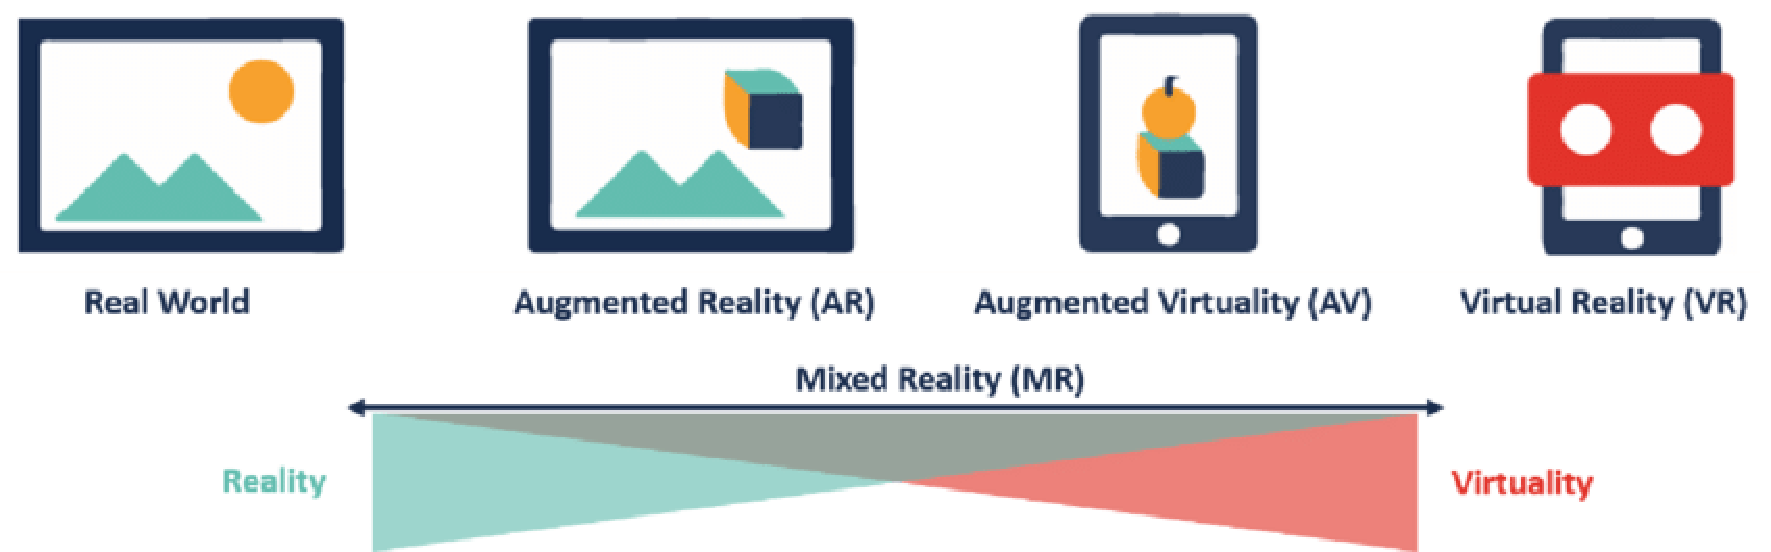
\includegraphics[width=14cm]{kapitel/eps/spectrum-of-reality.pdf}
  \centering
  \caption{Graphical representation of the dimensions of reality by 	  \cite{Lovreglio.2018}}
  \label{fig:spectrum}
\end{figure}

The reality describes the real world and using non digital devices for interaction, such as a steering wheel for driving a car for example. As mentioned in the indroduction, AR is a related technology to VR. In the spectrum of \cite{Tham.2018} AR covers the second level of reality dimensions. It describes computer generated elements, which are embedded into the reality. A famous example for an AR application is the game PokemonGo (\url{https://www.pokemongo.com/en-gb/}), in which players search in the real environment for computer generated items, based on a phone's camera and location services. The next level of reality is the augmented virtuality. This term describes a virtual environment, in which users can interact through analogue methods. An example for this could be a video chat room where the participants are present in a virtual room but communicate through analogue methods. As seen in figure \ref{fig:spectrum}, augmented reality and augmented virtuality can be summed up with the term \"mixed reality\" which describes the interaction between real life elements and the virtual environment. Finally, in the last stage there is VR in which a user is fully surrounded by a computer generated environment. This environment is most likely a reproduction of a real-life environment. The user is not only surrounded by an artificial reality but can also interact with it. It might happen that the user actually feels present in the virtual reality. In the following, this phenomenon will be explained in more detail.

\subsection{Immersion and storytelling}\label{immersion}
\todo{What is immersion and why so important for VR? What describes a good storytelling? Is there anything special when designing a story for a VR application?}
The term immersion often comes up when talking about VR. This term describes an experience which users would not be able to percieve without the use of the specific medium. In general, it describes an experience from a different point of view. This could be for example the story of a different character or the exploration of a unknown location. \cite{Tham.2018} \\ Immersion is an important measurement for this work. The experience, students have when playing the VR application, which will be developed during this thesis, depends on the grade of immersion.
When talking about immersion, it is important to distinguish between  mental and physical immersion. Mental immersion describes the state, in which the participant feels deeply emotionally connected to the virtual world. Physical immersion on the other hand means that the user's physical interactions are transferred into the virtual environment with the use of technology. The movements should feel as natural as possible to the user. When talking about immersion in books, films or related media, it is often only referred to mental immersion, because these types of media are not able to provide the technology for interacting with their environments. VR on the other hand can create immersion through a physical way as well. That is why VR can provide a higher grade of immersion than other media. \cite{Tham.2018}\\
Another term closely related to immersion is presence. Presence in the context of VR describes the subjective feeling of actually existing in the virtual world. The feeling of presence is a mix between mental and physical immersion. The more presence users feel, the more they accept the virtual world as the reality. To gain the sense of presence, the participant's movements in the reality should match with the movements of the virtual world. With a higher grade of presence, participants act more natural in a virutal environment, such as they would in a real environment. Through this, their task performance increases. This is one reason why presence is an important factor when it comes to developing VR applications, especially in the field of education and learning. \cite{Slater.1997}

Since the terms immersion and presence are explained, it is now the question, how to design the story of a VR application in order to gain a maximum grade of immersion. Storytelling is one of the most important elements for mental immersion in a virtual experience. Especially mental immersion can be influenced by the storyline, while physical immersion can be increased through hardware tools. \\
Storytelling in general is the art of telling a narrative to the user in a way that the user is not only consumer but actually feels immersed with the story \cite{Louden.2018}. Designing a storyline in VR opens a lot of possibilities in engaging the participant in the story. Therefore there are things to consider when it comes to storytelling in VR as explained by \cite{Keane.2018}:\\
One thing to bear in mind is, that space and environment in a VR application are more important than in other media, like books or films. The creator designs a world in a 360 degree view, so there is a lot more space to show. The storyline not only happens in front of the users, but can be all around them. Because the user is able to walk independently in the virtual world, it is very important to softly guide users into a certain direction when necessary for the storyline. The guidance should not be conspicuous, but should attract  users' curiosity. This can be achieved through light and sound effects or movements. Another aspect to consider is not to overwhelm  users with complex tasks. This could prevent the user in experiencing an immersed virtual world because their full attention would lie on completing the tasks.
\subsection{Interaction: Selection, manipulation and navigation}
\todo{different interaction tasks in VR and their common solution: Simple virtual hand, raycasting, go-go, HOMER, scaled world-grab, occlusion; describing ways of movement (walking aroung) solutions in VR}
In order to get an immerse experience, the user of a VR application needs to interact with the environment. When it comes to interaction in VR, several challenges occur. First of all, there is a three dimensional space which has to be covered. Secondly, when users are wearing the HMDs, they cannot see the controllers they are using in the real world. This means, that every hardware controlling device should be mapped into the virtual world. This chapter describes some typical interactions and their common solutions in VR. It is a base overview of interaction methods, which can be considered to be used in the prototype VR application. The final method, which suits the best for the prototype, will be discussed in chapter \ref{design}.\\
Basically, there are two different types of interaction in VR: Modifying the virtual world and moving in the virtual world. When modifying the virtual world, the user should be able to select and manipulate objects. Manipulating includes moving, scaling, changing of look (color, texture) and orientation of an object in the virtual world. When walking around in the virtual world, the user should be able to move freely and make their own decisions in navigation. \cite{Dorner.2013}\\
A challenge when finding solutions to the described interaction problems is, that there do not exist standard solutions, like we have in a screen based 2D context for example. Nevertheless, There are some best practices on how to implement the described requirements in VR. In the following, the most common interaction techniques will be explained according to \cite{Dorner.2013}.

A very straightforward method in selection could be the selection through gaze. The user can select objects by looking at it. This is a very simple method and works without hardware controllers for user input. An analogy in 2D interfaces would be the selection via mouse over. However, this technique does not work well in VR. The problem is, that users accidentally select objects every time they look around. A simple and natural exploring of the virtual world would be interrupted by object selection.\\
Another technique is called ray-casting. It works with a virtual virtual ray coming from the users' hand. Therefore, an controller or a hand tracking hardware is needed, which movements are mapped into the virtual world. Every object which collides with the ray is a possible candidate for selection. Most of the time, the object nearest to the user will be selected. ray-casting is an important method in object selection, because it is very straightforward and conforms to the expectations of users (TODO why?). Nevertheless, this method becomes inaccurate when to deal with large distances, because the movements of the hand has to be more accurate the longer the distance gets. \\
The next method, the Go-Go technique overcomes this problem. A virtual arm, mapped with the user's hand movements is displayed in the virtual world just as done with the ray-casting method. The difference of the Go-Go- technique is, that the virtual arm can be lengthened, if the selectable object is out of range. When the virtual arm is lengthened, the user's hand movements are mapped in a smaller range, than when the virtual arm is in the normal position. This mapping is not linear and overcomes the problem of inaccuracy when selecting objects to far away. The technique can be well used for relocating objects, because the user does not have to walk on the same time. However, with this technique, as well as with the ray-casting technique, only objects which are in viewing range can be selected or manipulated. Some objects could be overlapped by other obstacles and cannot be selected. Also, objects in far distance appear very small, which makes manipulation difficult.\\
The HOMER technique deals manipulation of objects in distance. The abbreviations stands for Hand-Centered Object Manipulation Ray-casting. As the names says, it uses techniques of the ray casting for selection. To make the manipulation easier, the object moves to the users hand, once selected. The user can now perform their desired manipulation. After the manipulation is finished, the objects teleports back to its original position. This technique still has the problem of selecting objects which are not in the user's viewing range.\\
\begin{figure}[h!]
  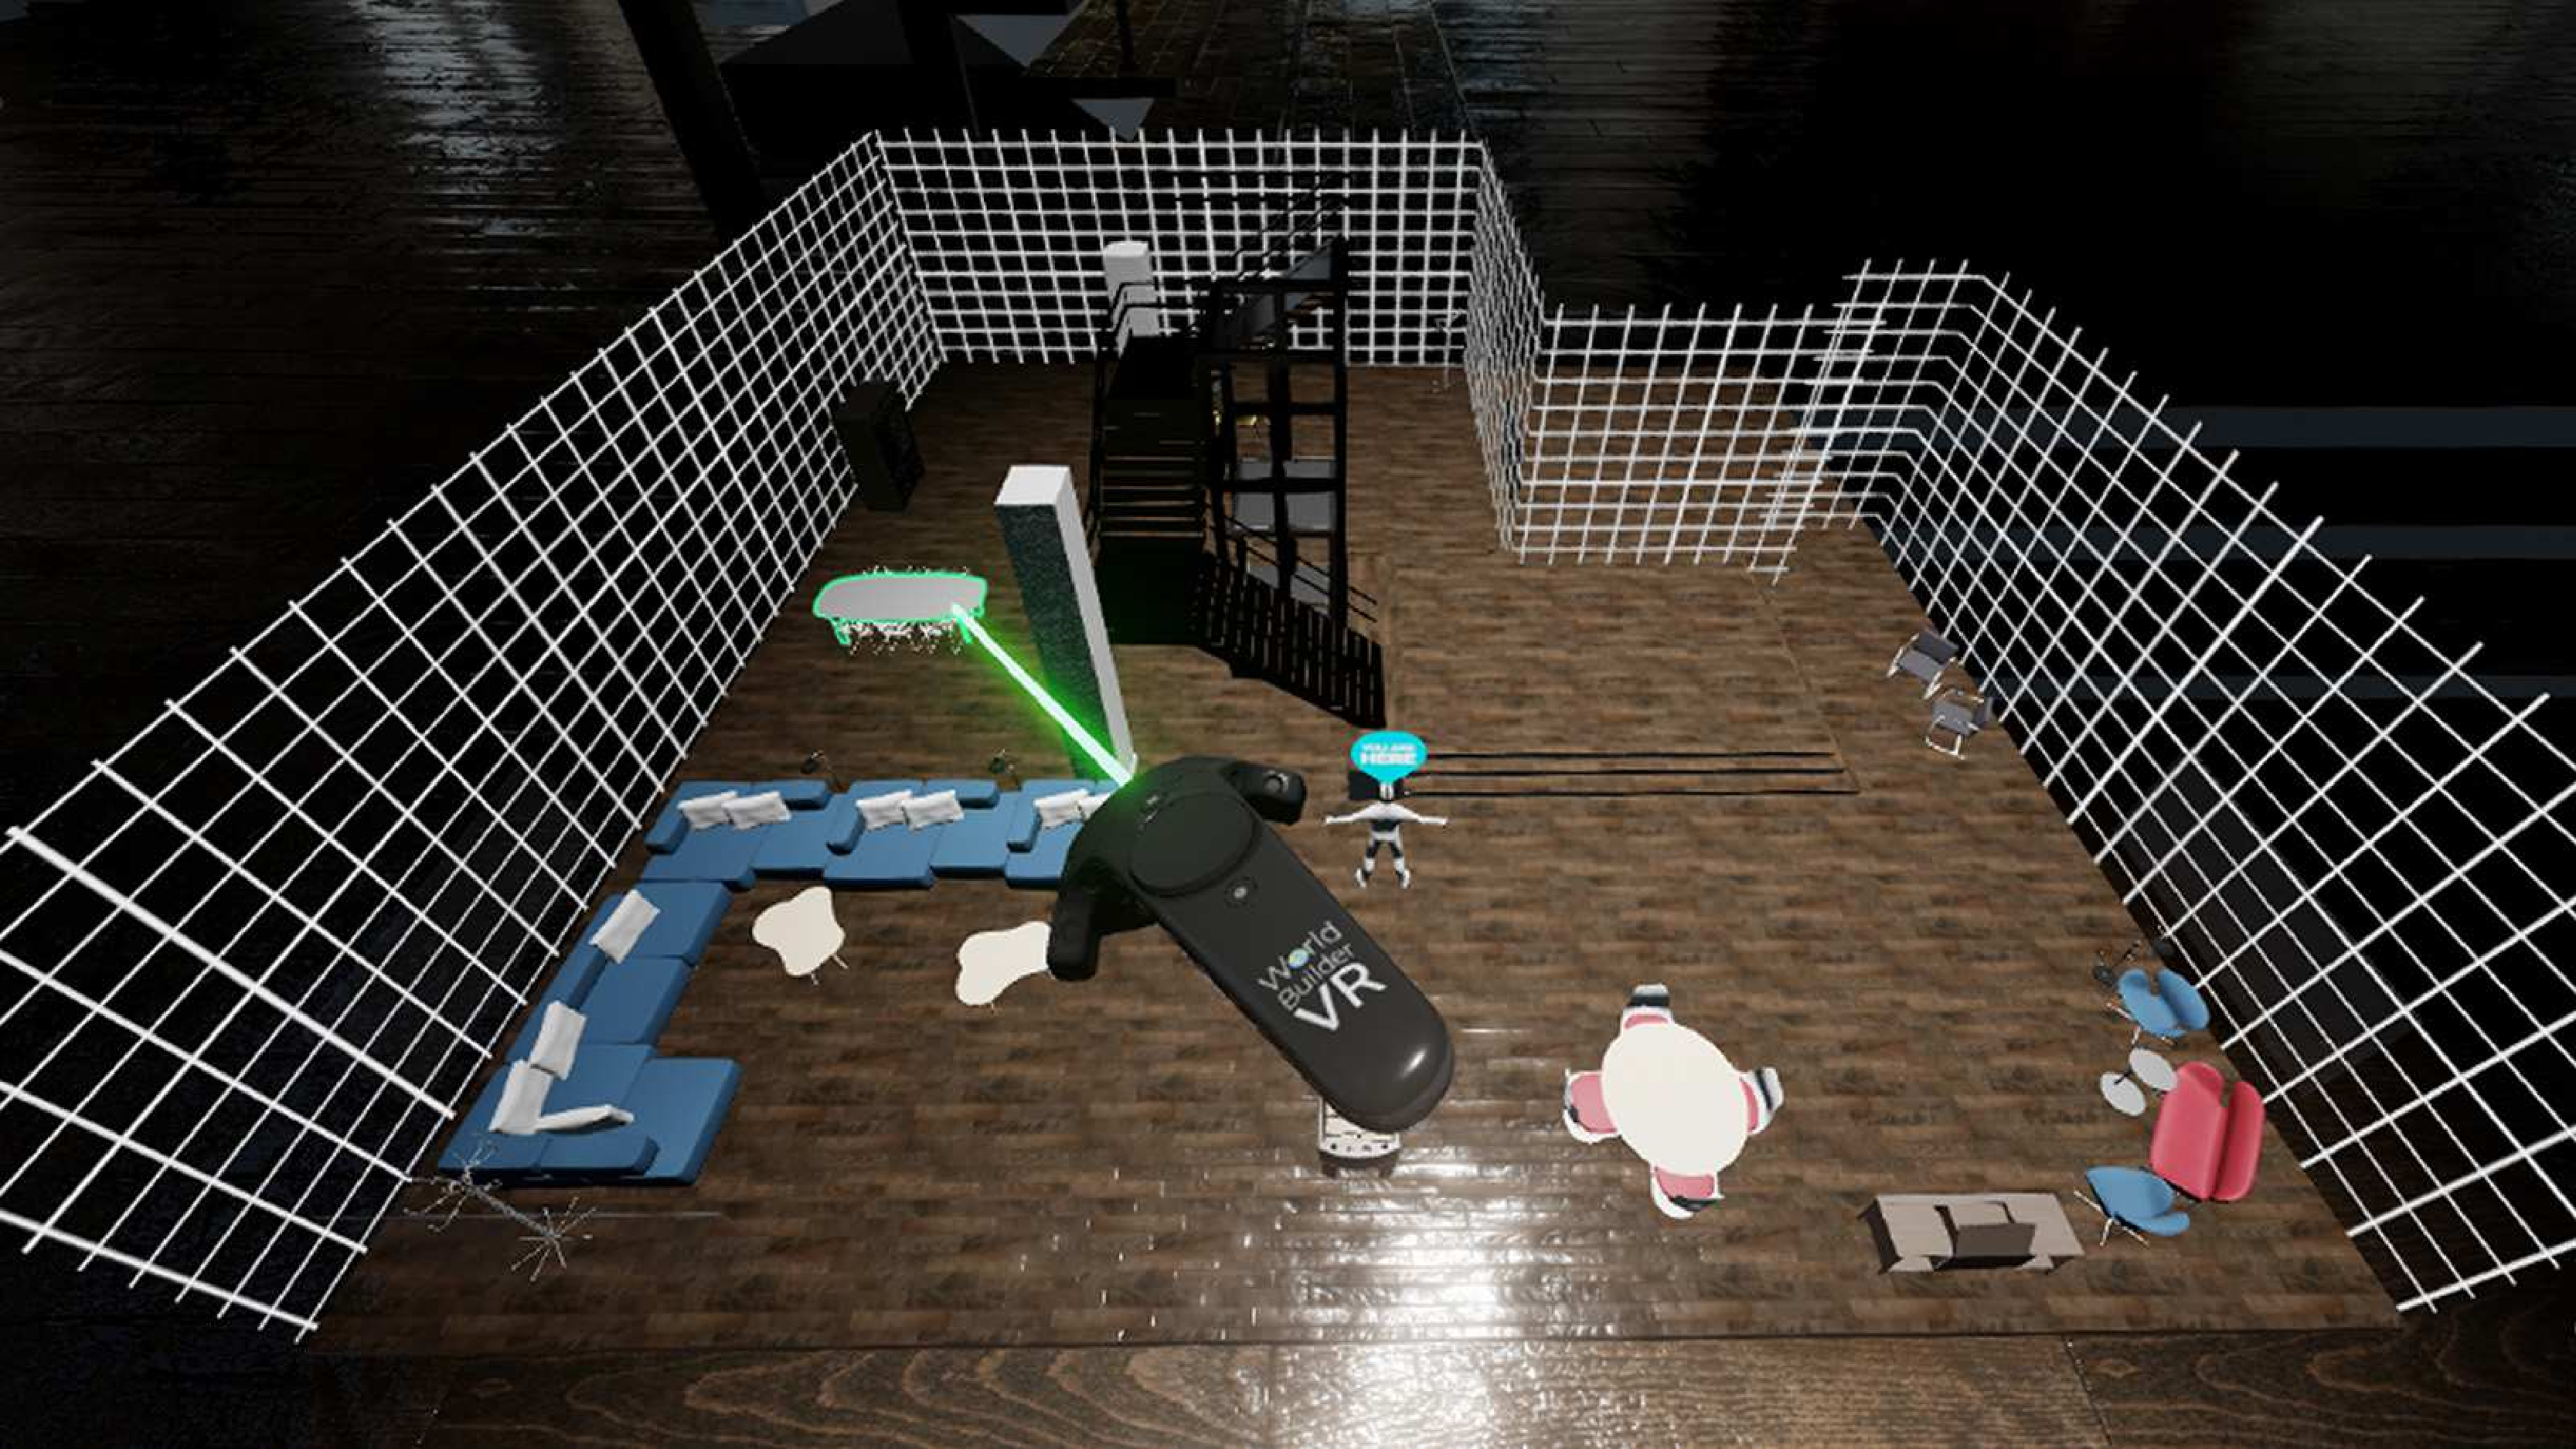
\includegraphics[width=14cm]{kapitel/eps/mini-map.pdf}
  \centering
  \caption{Mini map as part of the WIM technique. By \cite{Arnowitz.2017}}
  \label{fig:minimap}
\end{figure}
An alternative to this method is the world in miniature (WIM) technique. As seen in figure \ref{fig:minimap}, the user gets a miniature map of the virtual world with all selectable objects. The user can now select the desired object in the map and it gets highlighted in the virtual world. With this method, the user looses their ego centred point of view. This can be seen as a decrease in an immerse experience, although it increases usability.

When it comes to moving in the virtual world, the problem of only seeing the virtual world but not the physical world becomes more real. There is a danger of physical damage when colliding with real world object while wearing a HMD. There is a conflict between the real world limited space and the unlimited virtual world (TODO source). Therefore some techniques are described also by \cite{Dorner.2013} how to deal with the problems of navigating through virtual worlds:\\
One method of moving around in VR can be the direct manipulation of the camera with a suitable input controller. The user moves the camera with the help of a joystick for example. Another method, which is very common in 3D computer games and therefore conforms highly to the expectations of users, is the walking in the direction of the user's point of view. A disadvantage of this method is, that the user cannot look around while moving. Both described techniques have the disadvantage, that they can cause motion sickness. This phenomenon will be described in chapter \ref{limits}.\\
To overcome the motion sickness problem, a very common technique for navigation is teleporting. Teleporting means to translate the user directly to a specific position without a time delay. The technique can be realised in VR by selecting the desired translation point via ray-casting and jumping to the point after selection. This method successfully overcomes the problem of motion sickness, but there is a loss of immersion, since this kind of navigation is not very natural.  \cite{Bozgeyikli.2016}\\
The most natural and immerse way of navigating is physical walking. Walking in a virtual environment deals with all the problems of space and the above mentioned conflict between real and virtual world space. Natural walking in general needs more complex hardware for tracking the users movement than navigation with the help of a hand controller. One method of walking in VR is the walking in place method. As the name describes it, the user moves in the virtual world by lifting their legs but they are not actually changing their position in the real world. There are several hardware installations which support walking in place, some of them make walking possible through a treadmill like system.\\
It is also possible to let the user walk around in room which was designed for virtual reality usage and provides suitable tracking sensors. To avoid colliding with the real world borders of the room, the redirected walking technique was developed. With this technique it is possible to make the user believe they are walking straight, while small changes in the virtual world make them actually move in circles or in similar paths as seen in figure \ref{fig:walking}
\begin{figure}[h!]
  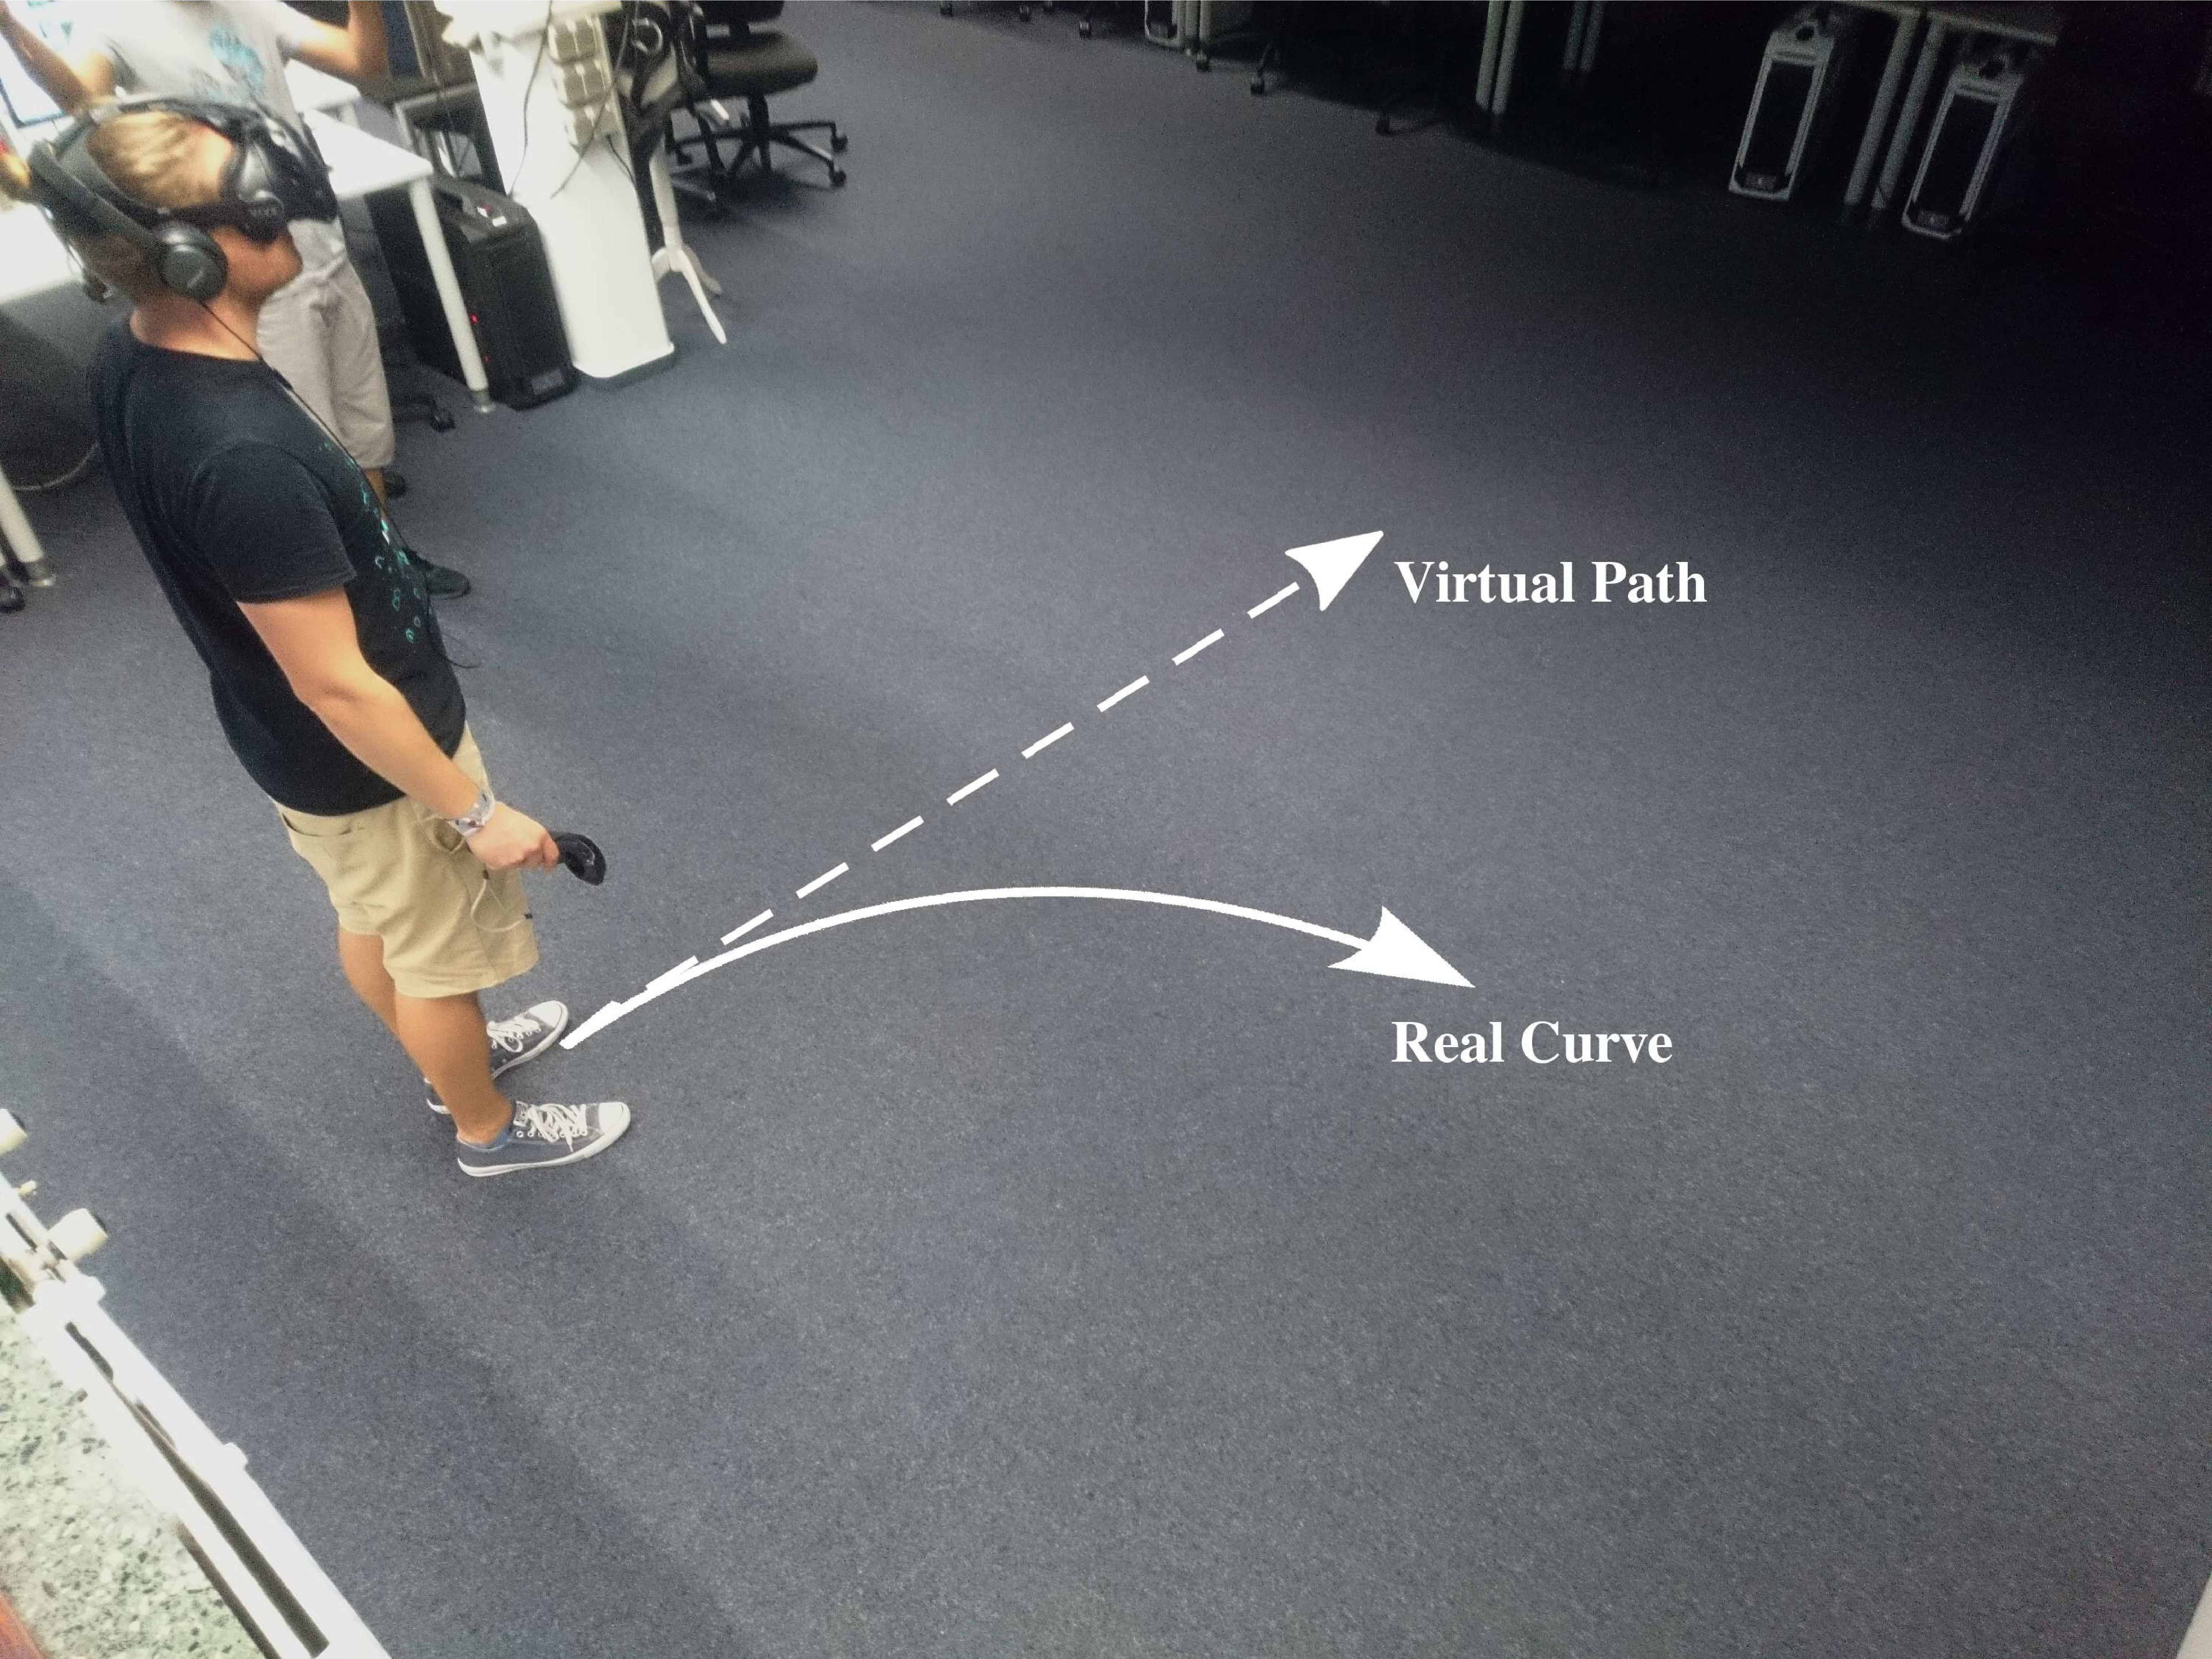
\includegraphics[width=10cm]{kapitel/eps/redirected-walking.pdf}
  \centering
  \caption{Redirected walking in VR, virtual walking path vs. actual walking path. By \cite{LS18}}
  \label{fig:walking}
\end{figure}

\section{Hardware for VR}
\todo{describe difference between mobile and desktop HMDs, show examples HTC Vive and Google Daydream, maybe also Google Cardboard. What possibilities of interaction do they provide?}
There has been a lot of research in hardware technologies to support physical immersion in VR. Some important objectives when it comes to new hardware technologies in VR are the increase of immersion, the reducing of costs and the decreasing of size and weight. The two main types of HMDs currently available are the desktop HMDs and the mobile HMDs. The first type runs the application on a standalone desktop and the HMD measures the sensorical data from the user. The second type uses the phone to run the application and the phone's sensors to measure head rotation and other relevant data. In general, the desktop HMDs have the better performance than the mobile HMDs because the processing of the game is transferred to a standalone desktop PC instead of a phone inside the HMD. \cite{Dorner.2013}\\
An addition third type of HMDs are the standalone devices, they are similar to mobile VR headsets but there is no need of attaching a mobile phone into the HMD. Instead, the device works out of the box. The performance of those standalone devices is lower than the desktop but higher than the mobile HMDs. \cite{http://www.isaca.org/Knowledge-Center/Blog/Lists/Posts/Post.aspx?ID=975&utm_referrer=direct%2Fnot%20provided/oculus-go-standalone-vr-headset-review
}\\
For this project, the game will be deployed on two different devices. The devices provided for development are the Samsung Gear VR headset and the Occulus Go headset. This chapter compares the two devices and point out their advantages and disadvantages. Both devices can be seen in figure  TODO. %\ref{fig:devices}.

\paragraph{Samsung Gear VR} Samsung Gear VR is a mobile based VR headset which was developed by Samsung and Occulus, introduced in 2017. The performance and screen resolution of the HMD depends on the mobile phone, used with the headset. Gear VR is currently supported only by the newer Samsung phones, including Galaxy S6 and higher, Galaxy Note 5 and higher, Galaxy A8 and higher.
It comes with a bluetooth hand-held controller which can either be held in the left or right hand. Inside the HMD is a gyro sensor to detect head rotation. There is a proximity sensor as well in the headset to detect if the user is currently wearing the HMD. The device does not support motion controlling. \cite{Samsung.2019}\\
Gear VR works intuitive with the supported devices and is supported by the game engine unity, which makes the software application development easier. However, the use of a Samsung mobile phone is required, and not all Samsung phones are supported.
\paragraph{Occulus Go}
This device was announced in May 2018 and is a standalone device. That means there is no need of an additional smartphone to be attached in the device.
Inside the HMD is instead a Qualcomm Snapdragon processor which is widely used in smartphones. The screen resolution is  2560 x 1440 pixel. This resolution is comparable to high class smartphones of the year 2018 and therefore comparable to the Gear VR in combination with a suitable smartphone. The sensors and the handheld controller are very similar to the Samsung Gear VR device.\\
Looking at the technical data, there is not so much of a difference between the two devices. Nevertheless, an advantage of the Occulus Go is, that no phone has to be attached to the device. Also the head strap and the audio output was improved.\cite{https://www.theverge.com/2018/5/1/17306458}
\section{Showcases of VR applications}
There are a variety of VR applications available for very different use cases and made with diverse concepts. The following chapter will present one VR application which is of the category of 360 degree videos, one application from the field of gaming and the last application will be about education and learning.
\section{Limits of VR} \label{limits}
\todo{At current status, what is VR not able to achieve? What are the challenges VR researchers face currently?}
The idea of VR is not a new invention of the past few years. There has already been a peek in research and also prominence to the public in the late 90's and beginning of 2000. However, the technology did not prevail in the economy, because there were several limitations especially in performance of computation. Therefore only a limited amount of ideas were able to be actually implemented. Another problem at that time were the very large and heavy HMDs (TODO insert image). The user could not wear them for a very long time and it caused neck pain and other physical problems. The devices were also not portable. \cite{Jerald.2016}\\
Looking at VR technologies now, a lot has changed. At first, the performace of our processors have increased rapidly. Secondly the HMDs became a lot smaller and lighter compared to the ones of the late 90's. But yet, we are not at the point, where all research is done -- on the contrary: A lot of challenges still occur when creating a VR application today. In the following, the problem of motion sickness will be explained. It will also be pointed out, what solutions are upcoming in the near future. There is also a lot of research in progress, when it comes to maximise physical immersion. It will be explained, what interactions cannot be covered by today's hardware, and what technologies are in development or testing at current stage.
\subsection{Motion sickness}
Motion sickness is a very common problem in VR. It can be compared to the kind of sickness, some people experience when being in moving vehicles, such as buses, cars or roller coasters. The symptoms are nausea, dizziness or even vomit. Most of the time this symptoms occur after a usage time of more than 10 minutes. Unfortunately, motion sickness does not occur on a very small percentage of people and therefore cannot be ignored easily. In the study of \cite{Siess.2017}, over a half of the test persons experienced one of the described symptoms during playing a VR roller coaster game.\\
The most likely reason for motion sickness in VR is the mapping between real movement and virtual movement. For example, there is a high propability of feeling sick, when there is a latency between head movement and the movement in the virtual world. This latency  will be registered by the brain and is experienced as unfamiliar and weird. Other situations, such as walking in the virtual world without physically moving can be a reason for motion sickness as well. \cite{Dorner.2013} \\ \cite{Siess.2017} also listed other reasons such as excessive speeds, for example first person moving speed or the moving speed of nearby obstacles, insufficient graphics or general technical problems( e.g. quality of lenses or comfort of HMD).
\cite{Fenlon.2013} mentions the removal of player control as a reason for motion sickness. It is more likely to experience the symptoms, if the games takes control over the head rotation instead of the player. \\
To overcome the problem of motion sickness, the latency between physical and virtual movement has to be as small as possible. This is of course limited by the performance of the hardware devices. Many creators try to manage the problem by creating short time experiences with less than 10 minutes durance and trying to avoid fast moving objects in their application. \cite{Doerner.2013}\\
This approach however, limits the possibilities of VR applications. It would be hard to create an action shooter without fast moving objects, for example. \\
Besides this constraints, there have been new hardware developments lately, which promise to solve the problem of motion sickness in VR. One of this hardware inventions is a device by \cite{?} with vibration motors attached to it. User wear a headband with the motors placed near to the ear. Everytime users move in the virtual world, the vibration motors provide a haptic feedback. According to \cite{?} this vibration should affect the vestibular system and deludes a movement to the brain. The gap between physical and virtual movement can be tricked in a way through the device. However, the headband is still a prototype and so far, the effects and reasons for it are a hypothesis. There have to be more clinical studies until a clear statement of the effectiveness can be made.\\
Looking at the VR prototype application, which will be developed during this work, the risk of motion sickness should be held to a minimum. To fulfill this requirement, a balance between a high level of immersion and the reducing of motion sickness has to be hold. How this is realized, will be described in chapter \ref{design} and \ref{implementaion}. If the requirement is fulfilled, will be reviewed in chapter \ref{testing}.

\subsection{Hardware}
There are several limitations in hardware devices when it comes to VR at the time of writing. First of all, the sensors of a HMD have to work very accurate. Also computation of the head movement and the virtual world movement has to be as fast as possible (see previous chapter). The display resolution is too low currently. Screen resolutions which are working well when it comes to desktop screens or mobile screens do not work so good in VR, because the lenses zoom the picture and the pixels become visible. \\
When looking at physical immersion, there are a lot of potential enhancements in providing the user a more natural way of interacting with the virtual world. Hand held controllers have to be used in with  the most commercial available HMDs. A body tracking system would provide more immersion, but requires very accurate sensors.
Relocating the player in the virtual world is also a challenge at the time of writing. In chapter ?? the use of treadmill system was already mentioned. The following section will present a current available VR treadmill for VR. Within this example the current limits of physical walking VR are explained.

In \cite{Cakmak.2014} the cyberith virtualizer is introduced. It is a device which supports natural walking in VR through the walking in place method. Users are wearing special shoes and lean into a belt system, which can be seen in figure TODO. The feet are sliding onto the surface and translated as a movement into the virtual world. The movement mapping is realized through various sensors which are placed into the ground floor of the treadmill. It is possible to use the cyberith virtualizer with controller specialized games, because the software of this treadmill is emulating controller input commands.\\
This device, however is not yet available on the consumer market. The company had problems of finding customers after announcing and presenting it in 2014. In 2016 they announced that they would concentrate on the B2B market and yet they are not in serial production in 2019. \citep{TODO}\\
The reasons for this could be the expensive price and also the large size of the device. The consumer market might not be ready yet for devices like that. This example shows how challenging it is for commercial companies to make innovations in VR. Therefore it is important to push public scientific research in VR further forward.

\section{Measurement of effectiveness of VR applications}
\todo{name existing questionnaires about immersion, explain why they do not cover all aspects which are required for this application}

\chapter{Design} \label{design}
In this chapter we focus on the prototype VR application which is implemented. Before starting with the development, the content of the application has to be set. Also the requirements of the application have to be clear. For which target group the application is developed? What is the storyline of the application? How will the application be used later on? In the following, we shortly introduce, what kind of process model we choose for the implementation. After that, we set the requirements and target group for the prototype. The application will have a fictive storyline, similar to a computer game. In order to design the story, we create a storyboard and present it in this chapter. Once the content is set, we take a look at designing a dialogue with the user and choose suitable user input methods.
\section{Process model}
The objective of this thesis is to develop and evaluate a prototype VR application to simulate the different IT courses offered at NYP. To handle a complex task like this, it is important to apply a suitable process model. The project is developed in a group of two people, therefore a model like SCRUM would not be suitable in this case. Nevertheless, we divided our project in iterations and did a review after the end of each iteration. For this project an iteration of six weeks is chosen. The review contains a presentation in front of the supervisor and two independent lecturers. They give feedback about the prototype and ideas for enhancement. Every week, there is a meeting with the supervisor, in which current problems are discussed and tasks are set. For organizing our tasks we use elements from the process model Kanban, because this model helps keeping an overview of the status and the progress of different tasks. We visualise the tasks as cards and display them on a board, which can be seen in  figure \ref{fig:board}. Each card has a description, an assignee and an importance level. The cards are put in different containers: To-do, in progress, ready for testing and done.\\
Each IT course, which is planned to be represented in the VR application will be treated separately. This means, that during an iteration, not more than one job role will be in focus of the design and development part.  
\begin{figure}[h!]
  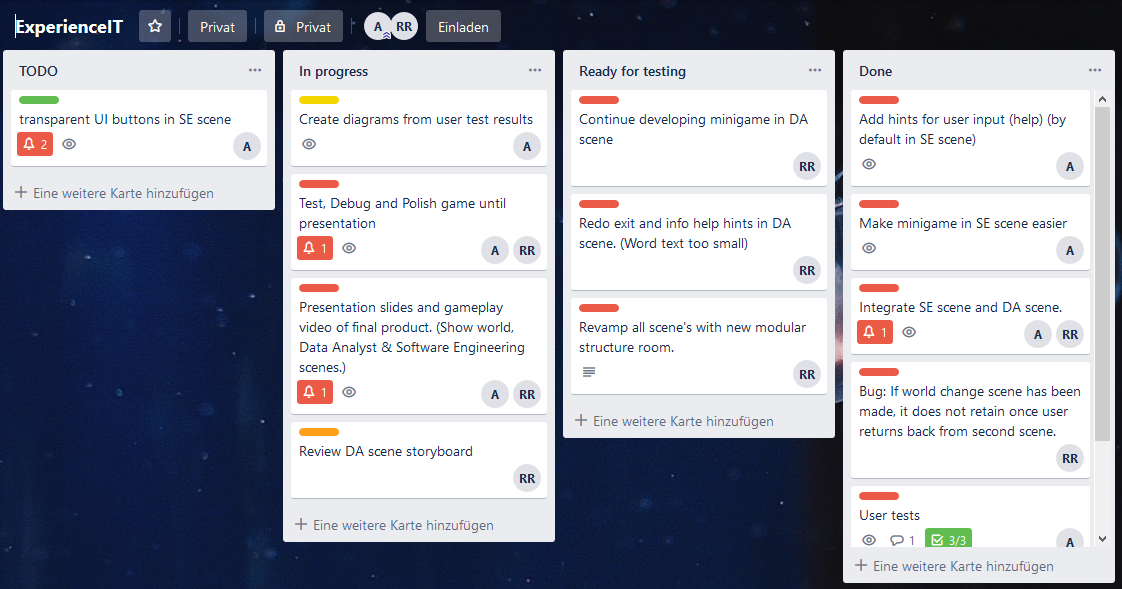
\includegraphics[width=16cm]{kapitel/kanban-board.png}
  \centering
  \caption{Board for visualising tasks and workflow.}
  \label{fig:board}
\end{figure}
\newpage
\section{Requirements}
In order to achieve the main objective of this work, several functional requirements have to be set:\\
\begin{itemize}
\item Introduction: The application should introduce the user to the various IT job roles.
\item Start scene: The application starts in a futuristic city which can be explored by the user.
\item Interaction: The user can interact with several objects in the starting scene and enter different scenes through this.
\item Separation: Each job role should be presented in a separate scene. The user should be aware of which job role the scene is referring to at all times.
\item Completing tasks: Each introduction of a job role should contain information of the job and a task which should be completed by the user.
\item Main storyline: There should be a main objective and each job role task is a step towards completing the main objective.
\item Gamification: The tasks should be structured as minigames and there should be a reward after completing them successfully.

\end{itemize}
Besides the functional requirements, there are several non-functional requirements which have to be considered when developing the prototype:
\begin{itemize}
\item Interesting: The user should gain more interest in the job roles introduced in the VR prototype.
\item Setting: The application should take place in a futuristic environment. Users should see how they can impact the future with IT.
\item Genre: The application should be a mix between a informative educational and a gaming application.
\item Educational: The user should gain more knowledge of the IT job roles after playing the VR application.
\item Portable: The application should be presented at various public events, such as open houses or fairs.
\item Budget: The product will not be distributed commercially. Therefore the costs for external tools, graphic or audio assets should be held to a minimum.
\end{itemize}

\section{Stakeholders}
In this chapter we define actors for the VR application. This is done by naming the different stakeholders of the application.
Stakeholders have different interests and expectations to the project. The \textbf{School of Information Technology} would like to have more students signing up for an IT course. They expect that the VR application arouses interest in IT by prospective students. Their task is to provide the application at public events, such as open houses and similar events. The School of Information Technology is also responsible for providing the IT courses which are introduced in the VR application. \\
The \textbf{project leader} expects a structured and well communicated application development. They expect that the objectives of the work is clear and the deadlines are met. The project leader is responsible for the guidance of the developers and the communication between the customer (School of IT) and the developers. The project leader sets and monitors the milestones in collaboration with the developers.\\
The \textbf{prospective students} are the end users of the VR application. They expect a joyful experience while using the application. They also want to learn more about the IT courses offered at NYP. Their task is to play the actual application. In case they are interested in one of the IT courses, they are responsible in applying for a diploma course at NYP.\\
The \textbf{developers} expect clear objectives from the project leader and a detailed description of the requirements. Their responsibility is to provide the actual application based on the frame given by the project leader and the customer. They develop a storyline, program the application and test it as well. In close communication with the project leader, they apply changes to the system.
\section{Target group}
Before starting with the design of the application, we have to define the target group. This makes developing of the application purpose easier and also helps keep the focus during the design process. A very important aspect of defining a target group is also, to develop the application directly to the needs of the future users. In the end this helps to increase the acceptance of the application. 

The main target group of the VR application will be prospective students, who are considering to sing up for a diploma course at NYP. As mentioned in the introduction, those students mostly come from a secondary school and have finished their O-Levels, which is an entry requirement for polytechnics. The secondary school educated the students on a very widespread basis, and the students can now decide their specialisation. \\
When the students leave their secondary school, the average age is 16. At this age, people are known to be open to new technologies and trends. The people in the target group are in the stage to make independent decisions for themselves without influence of parents. The application will be designed for prospective student which show an interest in information technology but yet have no experience or knowledge in that field.\\
In the following, a characteristic of a fictive person is displayed. This person stands as a representative for the target group of prospective students:

\paragraph{Characteristics}
\begin{description}
	\item[Name:] Jessica Lee
	\item[Age:] 16
	\item[Place of residence:] Singapore
	\item[Education:] Finished secondary school
	\item[Personal interests:] Dancing, computer games, TV series, technology
	\item[Level of tech experience:] Rich consumer, no programming skills
	\item[Expectation:] Wants to experience a fun virtual reality application
\end{description}
Since the fictive person Jessica Lee's main expectation is to experience a joyful application, there will be the need of gamification elements in the application. Her interests in computer games and technology lead the application's scene setting into a futuristic environment with new technologies. She has experience in digital media as a consumer, but not as a professional. Therefore, common gestures for user interaction can be applied, but the difficulty level of tasks about information technology should be on a beginner level. 
\section{Main story concept}
To gain the users attention and let them grow interest in the application it is important to have a good main story. The main story will create a bridge between the several IT courses displayed in the application. The story we present in this chapter is the main story line of the final product. We will only be able to realize parts of the main story in this work.\\
The VR application, hereinafter called game, will start in the so called ``Smart City''. This is a futuristic urban environment in which the user can move around freely. There are five different buildings along the streets. Each building is interactive and represents a course offered by NYP. When interacting with the buildings the user can enter laboratories, so called ``labs'', and complete different tasks. Every successful completion of a task has an impact to the main story. \\
The main goal of the game is to create a delivery drone which will deliver orders from online shops. This is still a vision of future for now, but it is a good showcase for the user to show them how they can impact the future with IT. During the completion of the labs several challenges will occur. Once the user started programming their first drone, a lot more drones will start flying around in Smart City. To avoid crashing and chaos, the next task is to provide a proper and stable internet connection to the drones, so they can communicate. But the connected drones have their advantages and disadvantages: At first they are flying normally and communicating to each other but then an unknown IoT-Hacker infiltrates a virus into the drone firmware, so they start to misbehave. Now the user has to trace the hacker with basic cyber security concepts. After the hacker was found, more and more inhabitants of Smart City start to use the drones and provide a lot of data. It is now the job of the user to analyse this data and optimise the drones. By combining relevant data, it is possible to add some enhancements to the drone.
Once the user completed all tasks and visited all labs, the user can exit the game. \\
During the development process of this work, it will not be possible to implement the whole main story and add all job roles. Instead, we will concentrate on one or two job roles. Other job professions will be added in an iterative process.
\newpage
\section{Storyboard}
In this chapter, we explain the structure and the details of the main storyline with the use of a storyboard. Since the requirements for the prototype application are already set, the storyboard points out the details of the requirements in a visual way.
The main objective of a storyboard is to get a scene by scene overview of the story and the sequence of events. Through a sketch draft, an idea of the visuals of the application is displayed. The focus of the storyboard lies on the storyline. Logical orders of scenes are displayed with arrows, textual explanations are added whenever necessary.\\
For the storyboard of the prototype, a tool called \textit{Invision freehand}\footnote{\label{foot:2} \url{https://www.invisionapp.com/feature/freehand}} is used. In the following, some important parts of the storyboard are presented \footnote{\label{foot:3} The complete storyboard can be seen in: \url{https://www.invisionapp.com/feature/freehandhttps://projects.invisionapp.com/freehand/document/Vbu2DFCdd}}. We introduced the IT courses from NYP in chapter
\ref{stateofart}. The final product should contain all job roles of the courses, but for the prototype in this work we focus our design on the job role of the software engineer scene and the cyber security specialist scene.
\subsection{World scene and software engineer scene}
\begin{figure}[h!]
  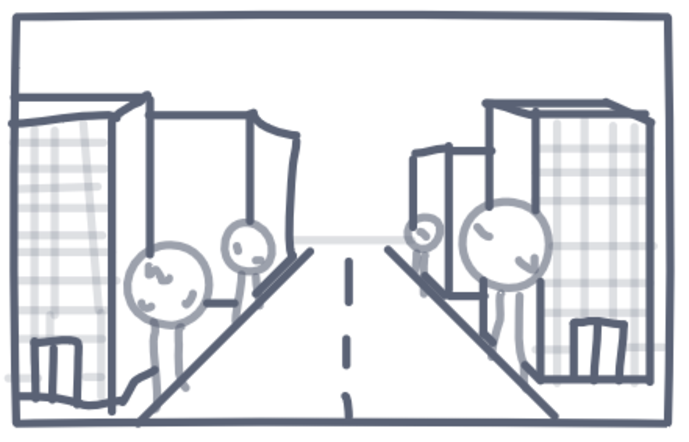
\includegraphics[width=8cm]{kapitel/storyboard/smart-city.pdf}
  \centering
  \caption{Smart city scene from where the user can explore different IT job roles (own illustration)}
  \label{fig:smartcity}
\end{figure}
The first scene of the storyboard is the smart city scene, as sketched in figure \ref{fig:smartcity}. Here the user can walk around freely. When the user selects the software engineer building, an assistant asks the user to enter the building. If the answer is ``yes", there is a transition into the software engineer lab scene. The lab contains a testing drone and a package as well as working desks with laptops. After the transition, the assistant explains the first task, as displayed in figure \ref{fig:sescene}. This is the first minigame, in which the user should gain understanding in how programming works.
\begin{figure}[h!]
  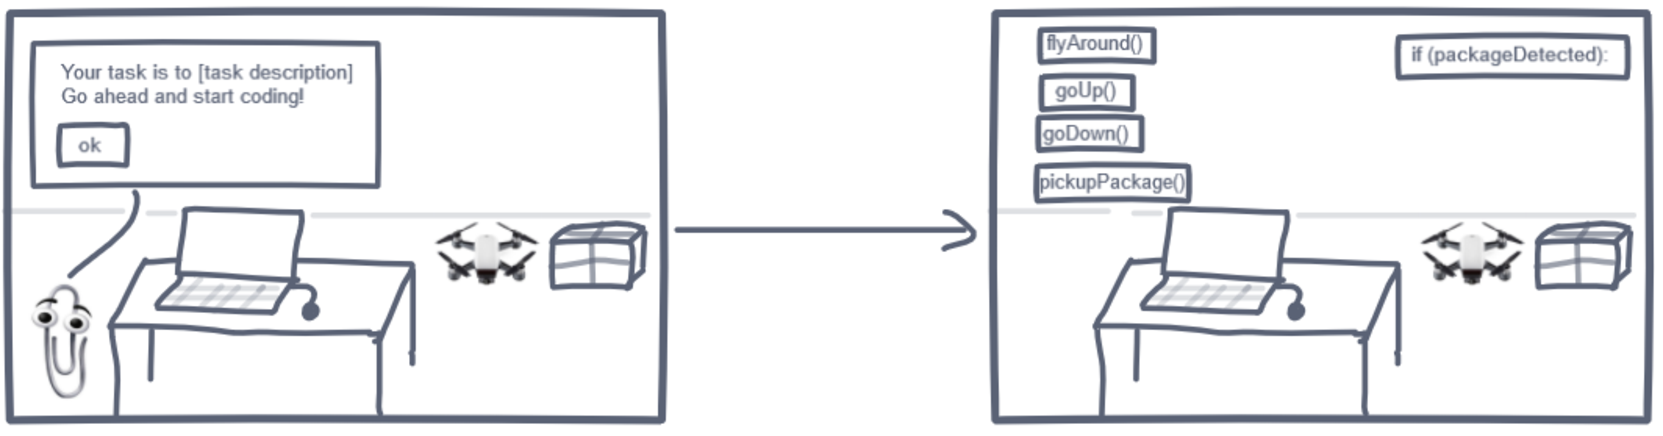
\includegraphics[width=16cm]{kapitel/storyboard/se-scene.pdf}
  \centering
  \caption{Software engineer scene: dialog and minigame (own illustration)}
  \label{fig:sescene}
\end{figure}
\\The information is taught in a very simplfied way, because the requirements of the application are that it should be playable without knowledge in IT. The objective of the task is to program the package delivery drone, so that it actually picks up a package. This is done by arranging lines of code in a logical order. The working environment is a desk with a laptop. After the user has arranged the code blocks and ran the code successfully, they can watch the testing drone in the lab picking up the package. With the completion of this minigame, the scene ends and the user is transferred back to the world scene.
\subsection{Cyber security specialist scene} 
The second scene represents the job role of the cyber security specialist. The scene is a laboratory with several office working places and the drone from the previous scene which is displayed on a table in the middle of the room. When the user enters the lab, they are informed that the drone they had programmed before was corrupted by an unknown hacker. During the next task, the user should gain knowledge in the methods cyber security specialists use to investigate digital crimes. The user learns about simple data decoding and encoding as well. The minigame is divided into three parts. 
\begin{figure}[h!]
  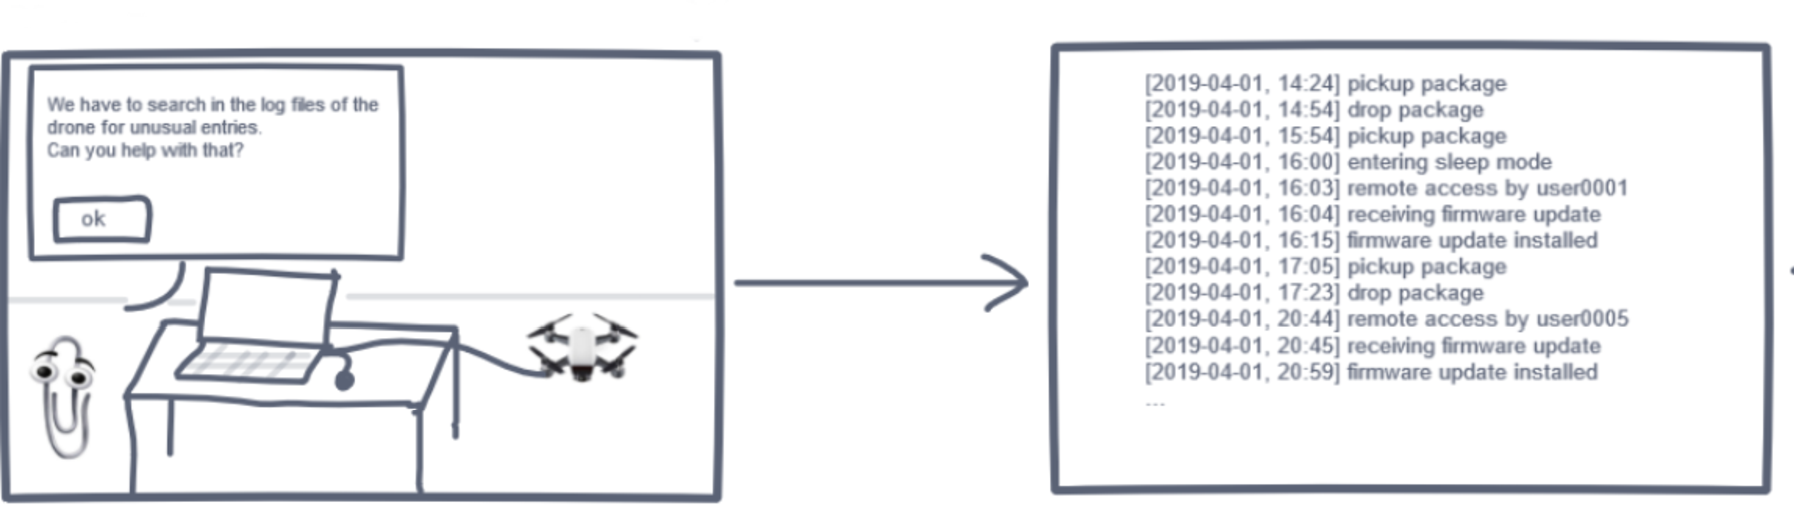
\includegraphics[width=16cm]{kapitel/storyboard/cyber-analyst1.pdf}
  \centering
  \caption{Cyber security specialist scene: searching log entries (own illustration)}
  \label{fig:logscene}
\end{figure}
\\In the first part, the user searches the log data of the drone for unauthorized access and marks suspicious entries which can be seen in figure \ref{fig:logscene}. It turned out that two lab employees have accessed the drone during the last 24 hours. in the second part of the minigame, users search the computers of the two lab employees for further information. 
\begin{figure}[h!]
  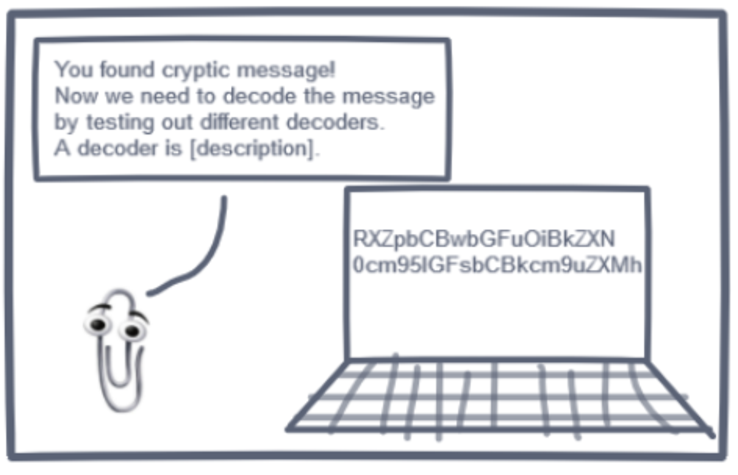
\includegraphics[width=8cm]{kapitel/storyboard/cyber-analyst3.pdf}
  \centering
  \caption{Cyber security specialist scene: encrypted message}
  \label{fig:logscene2}
\end{figure}
One employee has an encoded message on their desktop (figure \ref{fig:logscene2}).\\ Finally, in the last section, users decode the message by trying out different commonly used codes. The message reveals the hacker and the person can be prosecuted. This marks the end of the cyber security specialist scene.

%\section{Hardware evaluation}
%Looking at the requirements, one of the constraints for the application is, that it should be portable. Another requirement is, that the budget should be held to a minimum. This limits the number of hardware devices, which can be used within the VR application. When it comes to choosing a HMD, there is the decision between mobile HMD and desktop HMD. Since a mobile HMD fulfills the requirement of portability better than the dektop linked version, this is the preferred HMD.\\
\section{Dialogue design}
As seen in the storyboard, the application contains a lot of conversation between the assistant and the user. The dialogues are very important for the game, because they provide all the relevant information about the IT job roles. The dialogues should be presented in a natural and interesting way, because the application should arouse interest in IT job roles.\\
Spoken dialogue systems are the most natural way of communication, but on the other hand they are not easy to realise and need a lot of computation. This application will therefore stick with a text based dialogue system. To still provide a natural experience to the user, the dialogues should be mixed with interactions. Nevertheless, a voice over will be considered for the final product, but not for this prototype. \\
\begin{figure}[h!]
  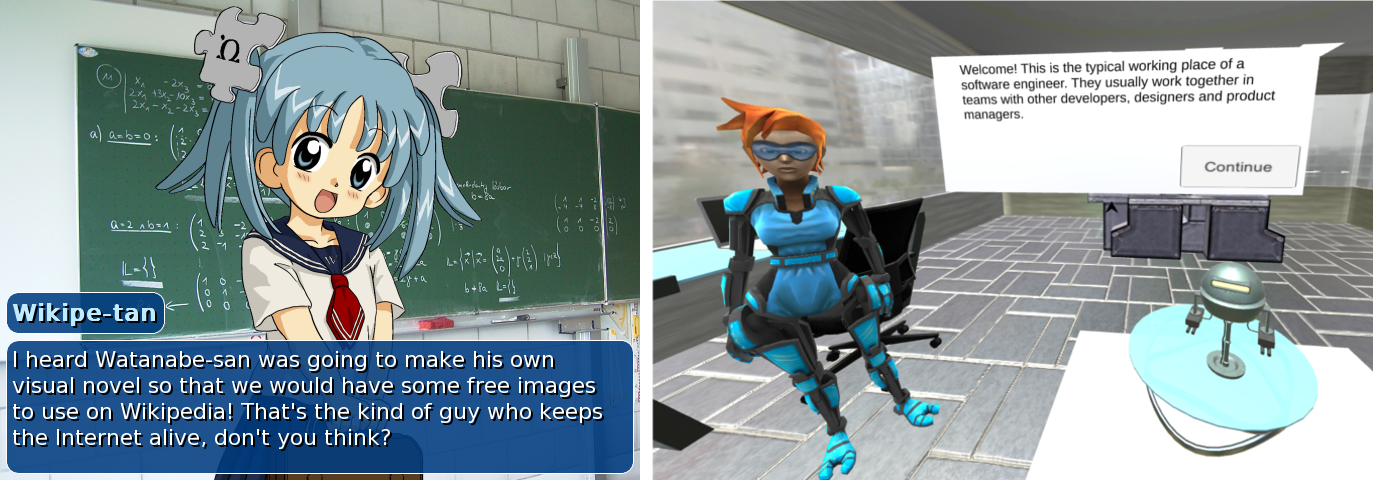
\includegraphics[width=16cm]{kapitel/screen-vs-world-dialog.png}
  \centering
  \caption{Screen space dialogue panel by \cite{screenspace} vs. world space dialogue panel.}
  \label{fig:screen-world-dialogs}
\end{figure}
When it comes to displaying the dialogue text in VR, there are some differences compared to a 2D space text displaying method. In 2D interfaces, for example in computer games, the conversation text of non playable characters (NPCs) is often displayed on the bottom of the screen and fixed to the screen space, like it is displayed in the left picture of figure \ref{fig:screen-world-dialogs}. This cannot be realised in the same way in VR. Users are not able to focus a screen space text when it is not directly in the middle of their view. Therefore, the dialogue texts are placed into the virtual world space, like seen in the right picture of figure \ref{fig:screen-world-dialogs}. The challenge of this method is to guide users to the position, where the dialogue is displayed. This is realised by placing the dialogue panel close to interactive items in the game. Once the user interacts with the items, the dialogue starts. The user is already focusing the objects and will notice the dialogue appearing in their view. Another method is used when there is a dialogue at the beginning of a new scene: The user's position and view is set close to the dialogue panel initially.
\section{User interactions}
In chapter \ref{stateofarts} we already introduced the different user interaction methods in VR that are commonly used. In this chapter we take a look at the different methods and evaluate, which method is the most suitable for the prototype VR application. There are several constraints and limitations in user interaction because of the hardware and the budget for the project. User interactions should also fit to commonly known user interactions like touch gestures or first person walking in computer games.\\
First of all we have to evaluate, what kind of user input Samsung Gear VR as well as Oculus Go provide out of the box.
The following input methods are available with the Samsung Gear VR: A wireless handheld controller or a touchpad attached to the HMD. Oculus Go provides a handheld controller which works the same way as the controller of Gear VR, but no touchpad at the HMD.\\
\begin{figure}[h!]
  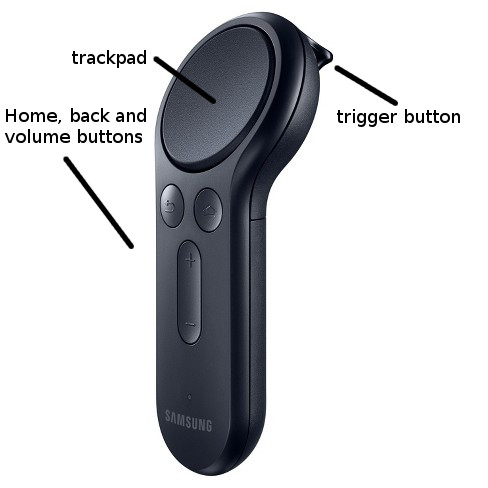
\includegraphics[width=10cm]{kapitel/samsung-controller.jpg}
  \centering
  \caption{Samsung Gear VR handheld controller \cite{Samsung.2019b}}
  \label{fig:samsung-controller}
\end{figure}
The handheld controller has gyro-sensors to detect its rotation but there is no position tracking. This means that the current controller  position is not mapped into the virutal world. As a workaround it is possible to reset the positioning of the controller with a button click.
The controller can either be used with the left or right hand. In order to use the controller, it has to be connected with the phone via bluetooth. To register user input, there are several buttons/trackpads, which are described in figure \ref{fig:samsung-controller}. The trigger button is a primary button, which can be pressed with the index finger. There is a trackpad which registers the thumb position and has a primary button as well. The last primary button is the back button. The controller registers the hand or arm rotation through sensors. There are home buttons and the volume buttons which are reserved by the system. The handheld controller of Oculus Go has the same buttons and functionalities, except the volume buttons which are located at the HMD directly.\\
The touchpad, located on the side of the HMD from Samsung Gear VR, registers touch position and touch gestures. Unlike the handheld controller, the touchpad does not need to be connected manually and always registers user input, when the HMD is used. It is therefore often used as a backup solution, in case no bluetooth controller is connected. However, the touchpad is only available for the Samsung Gear VR. We want the application to work with Oculus Go as well as with Samsung Gear VR. Therefore, the user input development is focused on the usage of the handheld controller.\\
Looking at the story board, several user interactions can be extracted:
\begin{itemize}
\item Relocating in the virtual world
\item Selection of objects
\item Relocating objects
\item Dialogue between assistant and user
\end{itemize}
First of all, we take a look at relocating in the virtual world, which is walking in VR in other words. Natural walking methods cannot be used because of missing hardware sensors. With the use of the handheld controller, the teleporting method or the camera manipulation method can be used. Since the target group are secondary students which are experienced in the usage of digital media, the method of the camera manipulation is chosen. It is expected, that the target group is already introduced to this kind of relocating, since it is widely used in computer games. To reduce the risk of motion sickness, the walking speed is held slow. The user can start walking when pressing the index trigger button. The direction of walking can be changed by moving the head.\\
The selection of objects is done with the help of the handheld controller. When using a controller, the ray-casting method is a very straightforward method for selecting. Ray-casting is also used in the default home application from Oculus. It is better to reuse well established user interface concepts than to introduce new input methods. Therefore, the ray-casting method is chosen for selecting objects in the VR prototype application. The implementation will be similar to the Oculus home application.\\
Relocating of objects is necessary when completing tasks. Especially during the minigame in the software engineer scene where the user has to arrange lines of code in order to code the software for the drone. To relocate the lines of code, the drag and drop method is chosen. By pointing and clicking on an object, it starts to follow the controller movements. Clicking again, the current position is applied to the object and its position is fixed in the world space. This is similar to a drag and drop action on 2D interfaces. Every object which has an interaction, will be highlighted when the user points with the controller at it.\\
The dialogue between user and the assistant is solved via a text based dialogue system, which is used in retro games for example. The user can control the dialogue flow and answer questions through simple button clicks.


%%%%%%%%%%%%%%%%%%%%%%%%%%%%%%%%%%%%%%%%%%%%%%%%%%%%%%%%%%%%%%%%%%%%%%%
% Literaturverzeichnis und Anhang
%%%%%%%%%%%%%%%%%%%%%%%%%%%%%%%%%%%%%%%%%%%%%%%%%%%%%%%%%%%%%%%%%%%%%%%
% Literaturverzeichnis auf einer ungeraden (rechten) Seite starten !
\cleardoublepage
%%%%%%%%%%%%%%%%%%%%%%%%%%%%%%%%%%%%%%%%%%%%%%%%%%%%%%%%%%%%%%%%%%%%%%
%  Literaturverzeichnis
%%%%%%%%%%%%%%%%%%%%%%%%%%%%%%%%%%%%%%%%%%%%%%%%%%%%%%%%%%%%%%%%%%%%%%
\refstepcounter{dummy}
\addcontentsline{toc}{chapter}{\refname}
%% Verschiedene Zitationsstile
% ITS
%\bibliographystyle{literatur/itsBibStyle}
% Sonstige
%\bibliographystyle{plaindin}
%\bibliographystyle{unsrtdin}
%\bibliographystyle{abbrvdin}
\bibliographystyle{alphadin}

%%%%%%%%%%%%%%%%%%%%%%%%%%%%%%%%%%%%%%%%%%%%%%%%%%%%%%%%%%%%%%%%%%%%%%
\bibliography{literatur/quellen}

% \input{kapitel/anhang.tex}

\end{document}
